%%%%%%%%%%%%%%%%%%%%%%%%%%%%%%%%%%%%%%%%%%%%%%%%%%%%%%%%%%%%%%%%
% Tipo de documento y paquetes
\documentclass[10pt]{book}
\usepackage{cdt/cdtAnalisis}
\usepackage{subfigure}
\usepackage{appendix}

%%%%%%%%%%%%%%%%%%%%%%%%%%%%%%%%%%%%%%%%%%%%%%%%%%%%%%%%%%%%%%%%
% Colores
\let\TAB\tabular
\renewcommand\tabular{\noindent\TAB}
\definecolor{gray1}{gray}{0.89}%{0.80}
\definecolor{gray2}{gray}{0.68}
\definecolor{gray3}{gray}{0.97}
\definecolor{pink1}{rgb}{1,0.87,0.75}
\definecolor{green1}{rgb}{0,0.75,0.75}
\definecolor{blue1}{rgb}{0.75,0.75,1}

%%%%%%%%%%%%%%%%%%%%%%%%%%%%%%%%%%%%%%%%%%%%%%%%%%%%%%%%%%%%%%%%
% Datos del proyecto
\sistema{Análisis del proceso de Gestión Escolar de la Escuela Libre de Derecho}

\proyecto[SAEV2.0]{Sistema de Administración Escolar V2.0}

\documento{Inicial}{Externo}{REING}{Propuesta del Nuevo Proceso de Admisión a Nivel Superior}{1.0}

\fecha{\today}

\organizacion{Escuela Libre de Derecho}

\author{Escuela Superior de Cómputo del IPN}

\elaboro[Líder de proyecto IPN-ESCOM]{M. en C. José Jaime López Rabadán.}   % Responsable del contenido (IPN)
\superviso[Área]{Persona.} % Quien recibe el documento (Contraparte)
\aprobo[Área]{Persona.} % Responsable Técnico (Contraparte)

\title{\varProyecto}
\subtitle {\varCveDocumento--\varDocumento}

%%%%%%%%%%%%%%%%%%%%%%%%%%%%%%%%%%%%%%%%%%%%%%%%%%%%%%%%%%%%%%%
% Elementos contenidos en el documento

% TODO: Al finalizar el análisis resuma aquí todos los elementos del componente: RN, CU, IU, MSG.
% \elemRefs{
% 	\elemItem{PU1}{1.0}{Proceso de Usuario 1, registro de nuevo Usuario}
% 	\elemItem{PPS1}{1.0}{Persona Física con Perfil Empresarial}
% }

%%%%%%%%%%%%%%%%%%%%%%%%%%%%%%%%%%%%%%%%%%%%%%%%%%%%%%%%%%%%%%%%
% Documentos relacionados con el documento actual
% TODO: Escriba los documentos en los que esta basado este documento.
\docRefs{
	\docItem{Reglamento General}{}{Reglameto General, Aprobado por la Asamblea Extraordinaria de la Junta General de Profesores, 19 de octubre de 2005. Última reforma, 27-V-2015}
	\docItem{Convocatoria de Ingreso}{}{Convocatoria de Selección a la Carrera de Abogado, Escuela Libre de Derecho, Ciclo Escolar 2017-2018 }
	\docItem{Introducción BPMN}{}{Stephen A. White. Introduction to BPMN. IBM Corporation}
	\docItem{Documentación BPMN}{}{Business Process Model and Notation (BPMN), v2.0. Número de documento en OMG: dtc/2009-08-14. URL de la documentación estándar: \url{http://www.omg.org/spec/BPMN/2.0/}. Agosto 2009}
	\docItem{F1.4-1}{1.0}{Formato de Datos Personales}
}

%%%%%%%%%%%%%%%%%%%%%%%%%%%%%%%%%%%%%%%%%%%%%%%%%%%%%%%%%%%%%%%%
% Inicio del Documento
\begin{document}

    %=========================================================
    % Portada
    \ThisLRCornerWallPaper{1}{cdt/theme/agua.jpg}
    \thispagestyle{empty}

    \maketitle
    
    %=========================================================
    % Hoja de revisión
    %\makeDocInfo
    %\bigskip\\
    %\makeElemRefs   --Coment--
    %\makeDocRefs
    %\makeObservaciones[3cm]
    %\vspace{2cm}
    %\makeFirmas

    %=========================================================
    % Indices del documento
    \frontmatter
    \LRCornerWallPaper{1}{cdt/theme/pleca.jpg}
    \tableofcontents
    \listoffigures
    %\listoftables
    \mainmatter

    %=========================================================
    % Para ocultar la información del documentador se descomenta: \hideControlVersion
    %\hideControlVersion
 
    %=========================================================
    % Capítulos del documento

    %---------- Introducción al contenido del documento
    %% introduccion.tex
%
% Describe el objetivo, alcance y contenido del documento.
%
%---------------------------------------------------------

%=========================================================
\chapter{Introducción}

\section{Objetivo del documento}

Objetivo
\noindent El presente documento tiene los siguientes objetivos:\\

\begin{objetivosDoc}
	\item Objetivos
\end{objetivosDoc}

%---------------------------------------------------------
\section{Alcance del documento}

Alcance. \\
\begin{UClist}
	\UCli { Generación de Convocatoria}.
\end{UClist}


%---------------------------------------------------------
\section{Organización del documento}
Organizacion

%---------------------------------------------------------
\section{Diagramas BPMN}

Los diagramas BPMN\footnote{Notación para el Modelado de Procesos de Negocio o BPMN por sus siglas en Inglés (Business Process Modeling Notation).} son una notación gráfica estandarizada que permite el modelado de procesos de negocio en un formato de flujo de trabajo, el objetivo es proporcionar una notación estándar que sea fácilmente legible y entendible por parte de todos los involucrados e interesados del negocio\footnote{Para más información sobre BPMN, revisar los documentos IntroBPMN y DocBPMN.}.\\

\noindent Los diagramas BPMN, a diferencia de los diagramas de flujo, permiten modelar el flujo de información entre diversas áreas y organizaciones, el tiempo que toma realizar cierta tarea y los productos generados. Por lo que se determinó la conveniencia de modelar el proceso de admisión de lass \cdtRef{Actor:EscuelaLibreDeDerecho}{Escuela Libre de Derecho} a través de este estándar.

%\noindent Los diagramas BPMN tienen la característica de mostrar la interacción existente entre las diferentes áreas, entidades o actores de la organización, esto permite visualizar el flujo de la información a través de las áreas.\\

%---------------------------------------------------------
\subsection{Procesos, Subprocesos y Tareas}

{\bf Proceso.} Es una serie de actividades (coordinadas u organizadas) bien definidas, que se realizan (alternativa o simultáneamente) bajo ciertas circunstancias con un fin determinado. Un proceso puede involucrar: ninguno o más de un {\bf subproceso} y una o varias {\bf tareas}.\\
% 	\begin{figure}[!h]
% 	\centering\noindent{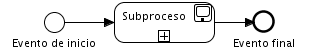
\includegraphics[width=225pt]{images/procesos/bpmn/CollapsedSubprocess.png}}%
% 	\caption{Diagrama de un proceso.}
% 	\label{Intro:CollapsedSubprocess}
% 	\end{figure}

{\bf Subproceso.} Es muy similar al {\bf proceso}, con la única diferencia de que éste sólo puede existir o suceder dentro de un proceso. Está representado por la Figura \ref{Intro:iProceso}.\\
 	\begin{figure}[!h]
 	\centering\noindent{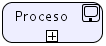
\includegraphics[width=71pt]{images/procesos/SubProceso}}%
 	\caption{Representación de un Proceso y/o Subproceso.}
 	\label{Intro:iProceso}
 	\end{figure}
% 	\begin{figure}[!h]
% 	\centering\noindent{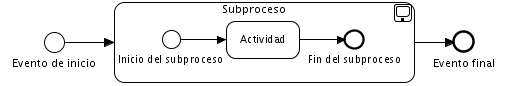
\includegraphics[width=360pt]{images/procesos/bpmn/ExpandedSubprocess.png}}%
% 	\caption{Diagrama de un subproceso expandido.}
% 	\label{Intro:ExpandedSubprocess}
% 	\end{figure}

{\bf Tarea o Actividad.} Es el grado de especificación más simple de un proceso (i.e; es el máximo detalle al que puede llegar un proceso) y de ella no pueden derivar más subprocesos o tareas. Está representado por la Figura \ref{Intro:iTarea}.
 	\begin{figure}[!h]
 	\centering\noindent{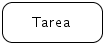
\includegraphics[width=68pt]{images/procesos/Tarea}}%
 	\caption{Representación de una Tarea.}
 	\label{Intro:iTarea}
 	\end{figure}
% 	\begin{figure}[!h]
% 	\centering\noindent{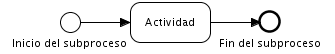
\includegraphics[width=240pt]{images/procesos/bpmn/SubprocessDiagram.png}}%
% 	\caption{Diagrama de un subproceso colapsado.}
% 	\label{Intro:CollapsedSubprocess}
% 	\end{figure}


%---------------------------------------------------------
\subsection{Subprocesos expandidos y contraídos}

{\bf Subproceso expandido.} Los subprocesos en BPMN, pueden representarse como se muestra en la Figura \ref{Intro:ExpandedSubprocess}. Esto significa que un subproceso puede contener varias actividades o subprocesos ``hijos''.
	\begin{figure}[!h]
	\centering\noindent{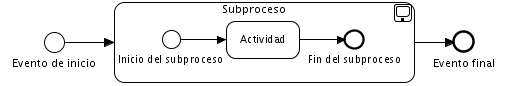
\includegraphics[width=360pt]{images/procesos/bpmn/ExpandedSubprocess.png}}%
	\caption{Subproceso expandido.}
	\label{Intro:ExpandedSubprocess}
	\end{figure}

{\bf Subproceso contraído.} Los subprocesos en BPMN, también pueden representarse como se muestra en la Figura \ref{Intro:CollapsedSubprocess}. Esta representación significa lo mismo que la Figura \ref{Intro:ExpandedSubprocess}, pero sin mostrar explícitamente sus actividades o subprocesos ``hijos''.
	\begin{figure}[!h]
	\centering\noindent{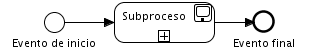
\includegraphics[width=260pt]{images/procesos/bpmn/CollapsedSubprocess.png}}%
	\caption{Subproceso contraído.}
	\label{Intro:CollapsedSubprocess}
	\end{figure}

% {\bf Diagrama de un subproceso.} Los subprocesos en BPMN, también pueden representarse como en la Figura \ref{Intro:ExpandedCollapsed}. Esta representación significa lo mismo que la Figura \ref{Intro:ExpandedSubprocess}, pero sin mostrar explícitamente sus actividades o subprocesos ``hijos''.
% 	\begin{figure}[!h]
% 	\centering\noindent{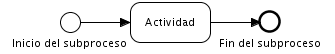
\includegraphics[width=360pt]{images/procesos/bpmn/SubprocessDiagram.png}}%
% 	\caption{Intro:Activity}
% 	\label{Intro:CollapsedSubprocess}
% 	\end{figure}


%---------------------------------------------------------
\subsection{Eventos}

Un {\bf evento} en BPMN representa algo que sucede o podría suceder durante el curso de un proceso y que afecta su flujo. Existen diferentes tipos de eventos:

\begin{itemize}
	\item {\bf Eventos iniciales}. Estos eventos inician el flujo del proceso y no tienen flujos de entrada.

	\arrayrulecolor{white}%
	\begin{tabular}{| m{.08\textwidth} m{.77\textwidth} | }% %{| c{.08\textwidth}  c{.77\textwidth} | }%
		\rowcolor[gray]{0.97}%
		\centering\noindent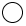
\includegraphics[width=18pt]{images/procesos/bpmn/StartEvent.png} & {\bf Evento inicial simple}. No se especifica algún comportamiento en particular para empezar un proceso. \\
		\centering\noindent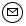
\includegraphics[width=18pt]{images/procesos/bpmn/MessageEventStart.png} & {\bf Evento inicial de mensaje}. Un proceso empieza cuando un mensaje es recibido. \\
		\rowcolor[gray]{0.97}%
		\centering\noindent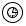
\includegraphics[width=18pt]{images/procesos/bpmn/TimerEventStart.png} & {\bf Evento inicial de tiempo}. Un proceso empieza en determinada fecha o tiempo específico.
	\end{tabular}%

	\item {\bf Eventos intermedios}. Indican que algo ocurre o podría ocurrir en alguna parte del proceso (desde el inicio y hasta el final). Estos eventos pueden ser usados como parte del flujo de secuencia o adjuntarse a los bordes de una actividad para indicar que la actividad se ejecuta una vez que el evento es activado.

	\arrayrulecolor{white}%
	\begin{tabular}{| m{.08\textwidth} m{.77\textwidth} | }%
		\rowcolor[gray]{0.97}%
		\centering\noindent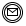
\includegraphics[width=18pt]{images/procesos/bpmn/MessageEvent.png} & {\bf Evento intermedio de mensaje}. Indica que un mesaje puede ser enviado o recibido en alguna parte del proceso. \\
		\centering\noindent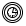
\includegraphics[width=18pt]{images/procesos/bpmn/TimerEventIntermediate.png} & {\bf Evento intermedio de tiempo}. Indica que el proceso debe esperar un tiempo especifico para poder continuar.\\
		\rowcolor[gray]{0.97}%
		\centering\noindent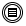
\includegraphics[width=18pt]{images/procesos/bpmn/ConditionalIntermediateEvent.png} & {\bf Evento intermedio de condición}. Se usa cuando el flujo necesita esperar por una condición de negocio para ser completado. Sólo puede usarse dentro de la secuencia del flujo o adjuntado a los bordes de una actividad para indicar que existe un flujo de excepción. \\
		\centering\noindent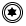
\includegraphics[width=18pt]{images/procesos/bpmn/MultipleIntermediateEvent.png} & {\bf Evento intermedio múltiple}. Este evento puede ser activado por muchas causas o sólo por una de ellas. Sólo puede usarse dentro de la secuencia del flujo.\\
		\rowcolor[gray]{0.97}%
		\centering\noindent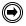
\includegraphics[width=18pt]{images/procesos/bpmn/LinkIntermediateEvent.png} & {\bf Evento intermedio de condición}. Este evento permite conectar dos secciones del proceso y puede ser usado únicamente dentro del flujo del proceso.\\
		\centering\noindent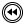
\includegraphics[width=18pt]{images/procesos/bpmn/CompensationIntermediateEvent.png} & {\bf Evento intermedio de compensación}. Permite manejar compensaciones. Puede ser usado dentro de la secuencia del flujo para indicar que se requiere una compensación, o adjuntado a los bordes de una actividad para indicar que la actividad será compensada una vez que el evento sea activado.
	\end{tabular}%

	\item {\bf Eventos finales}. Estos eventos finalizan el flujo del proceso, por lo tanto no pueden tener flujos de salida.

	\arrayrulecolor{white}%
	\begin{tabular}{| m{.08\textwidth} m{.77\textwidth} | }%
		\rowcolor[gray]{0.97}%
		\centering\noindent
\includegraphics[width=18pt]{images/procesos/bpmn/EndEvent.png} & {\bf Evento final.} Indica que el proceso y todas las actividades terminan, sin importar que alguna haya quedado pendiente. \\
		\centering\noindent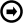
\includegraphics[width=18pt]{images/procesos/bpmn/LinkEvent.png} & {\bf Evento final de liga}. Este evento permite conectar dos secciones del proceso. Sólo puede usarse dentro del flujo del proceso.\\
		\centering\noindent
\includegraphics[width=18pt]{images/procesos/bpmn/CancelEndEvent.png} & {\bf Evento final de cancelación}. Permite enviar una excepción de error cuando el flujo llega al final. Este evento solo puede usarse en subprocesos.
	\end{tabular}%
\end{itemize}

%---------------------------------------------------------
\subsection{Compuertas}

Las {\bf compuertas} son elementos usados para controlar la divergencia y convergencia del flujo (separar y unir).\\

	\arrayrulecolor{white}%
	\begin{tabular}{| m{.08\textwidth} m{.77\textwidth} | }%
		\rowcolor[gray]{0.97}%
		\centering\noindent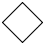
\includegraphics[width=25pt]{images/procesos/bpmn/ExclusiveGateway.png} & {\bf Compuerta exclusiva basado en los datos}. Como decisión exclusiva, tiene dos o más flujos de secuencia alternos, pero solo uno de ellos puede tomarse basado en la condición de los datos. Como convergencia, es usado para mezclar rutas alternas en una sola. \\
		\centering\noindent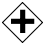
\includegraphics[width=25pt]{images/procesos/bpmn/ParallelGateway.png} & {\bf Compuerta paralela}. Como divergencia, es usada para crear rutas paralelas. Como convergencia, sincroniza multiples rutas paralelas en una. El flujo continúa cuando todas las rutas alcanzan la compuerta. \\
		\rowcolor[gray]{0.97}%
		\centering\noindent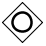
\includegraphics[width=25pt]{images/procesos/bpmn/InclusiveGateway.png} & {\bf Compuerta inclusiva}. Como divergencia, es usada cuando en un punto del flujo una o más rutas puden ser activadas y la decisión está basada en los datos del proceso. Como convergencia, indica que las rutas activas son sincronizadas en una sola.
	\end{tabular}%

%---------------------------------------------------------
\subsection{Conectores}

Los {\bf conectores} son elementos usados para conectar objetos (tareas, subprocesos, eventos, compuertas, etc.) dentro del flujo.\\

	\arrayrulecolor{white}%
	\begin{tabular}{| m{.33\textwidth}  m{.52\textwidth} | }%
		\rowcolor[gray]{0.97}%
		\centering\noindent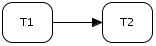
\includegraphics[width=120pt]{images/procesos/bpmn/SequenceFlow.png} & {\bf Flujo de secuencia}. Representa el control del flujo y la secuencia de las actividades, compuertas y eventos. \\
		\centering\noindent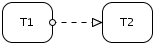
\includegraphics[width=120pt]{images/procesos/bpmn/MessageFlow.png} & {\bf Flujo de mensaje}. Es usado para mostrar el flujo de mensajes entre dos entidades o procesos. Representa señales o mensajes, {\bf no el control del flujo}. {\bf No todos los flujos de mensaje son secuenciales o esto especificaría orden en los mensajes}.
	\end{tabular}%


%---------------------------------------------------------
\subsection{Contenedores}

Un {\bf contenedor} es un elemento utilizado en BPMN para distinguir visualmente las responsabilidades entre las áreas u organizaciones.\\

	\arrayrulecolor{white}%
	\begin{tabular}{| m{.33\textwidth}  m{.52\textwidth} | }%
		\rowcolor[gray]{0.97}%
		\centering\noindent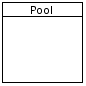
\includegraphics[width=45pt]{images/procesos/bpmn/Pool.png} & {\bf Pool}. Un {\it pool} es un contenedor representando un sólo proceso. \\%El nombre del {\it pool} puede ser considerado el nombre del proceso. \\
		\centering\noindent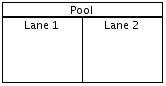
\includegraphics[width=70pt]{images/procesos/bpmn/Lane.png} & {\bf Lane}. Un {\it lane} es una subdivisión de un {\it pool} y representa un rol o área organizacional.
	\end{tabular}%

%---------------------------------------------------------
\subsection{Tipos de subprocesos}

%El {\bf proceso RENIECYT} describe una parte de la funcionalidad del registro RENIECYT, por medio de una serie de actividades bien definidas, con el objetivo de realizar el registro de los usuarios en RENIECYT.\\

Se han dividido los procesos de la \cdtRef{Actor:EscuelaLibreDeDerecho}{Escuela Libre de Derecho} en diversos subprocesos con la finalidad de entender y visualizar mejor su funcionalidad. Estos subprocesos se han clasificado en dos tipos:
\begin{itemize}
	\item Críticos. Son aquellos subprocesos complejos que pueden involucrar más de un subproceso y/o tareas y describen una parte sumamente importante del proceso propuesto para la \cdtRef{Actor:EscuelaLibreDeDerecho}{Escuela Libre de Derecho}. Están representados por la Figura \ref{Intro:iProcesoComplejo}.
	\begin{figure}[!h]
	\centering\noindent{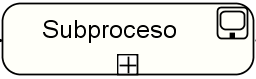
\includegraphics[width=71pt]{images/procesos/SubProcesoComplejo}}%
	\caption{Representación de un Subproceso Complejo.}
	\label{Intro:iProcesoComplejo}
	\end{figure}

	\item Simples. Son subprocesos sencillos y probablemente requieran únicamente de tareas para describir sus actividades. Están representados por la Figura \ref{Intro:iProceso}.
\end{itemize}

\noindent Notese que la única diferencia entre ambos es el color de relleno, los subprocesos críticos son de color amarillo, mientras que los subprocesos simples son de color azul.\\

%\noindent El proceso RENIECYT puede llevar a cabo diversas actividades las cuales pueden ser subprocesos o tareas. Se usa la Figura \ref{Intro:iProcesoComplejo} para indicar que una actividad es un subproceso crítico, la Figura \ref{Intro:iProceso} para indicar que una actividad es un subproceso simple y la Figura \ref{Intro:iTarea} para indicar que una actividad es una tarea.


%---------------------------------------------------------
\subsection{Nombre de los subprocesos}

\noindent Se usa la siguiente estructura para nombrar los subprocesos de Admisión de la \cdtRef{Actor:EscuelaLibreDeDerecho}{Escuela Libre de Derecho}:
	\begin{center}
		{\bf PP- + Tipo de Proceso + Número consecutivo + Nombre del subproceso}
	\end{center}

\noindent Donde:
\begin{itemize}
	\item{\bf PP-}. Significa que es un subproceso propuesto.
	\item{\bf Tipo de Proceso}. Puede tomar uno de los siguientes valores:
		\begin{itemize}
			\item{\bf A}. Significa que es un subproceso de Admisión.
		\end{itemize}
	\item{\bf Número consecutivo}. Estará dado por el nivel de profundidad que presente dicho subproceso. Por ejemplo, en la Figura \ref{Intro:JerarquiaProcesos} el Proceso General tiene un subproceso 1 y un subproceso 2.
		\begin{figure}[!h]
		\centering\noindent{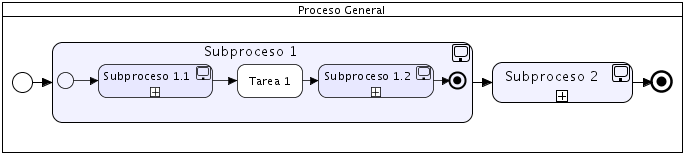
\includegraphics[width=0.87\textwidth]{images/procesos/JerarquiaProcesos_1}}%
		\caption{Subproceso General.}
		\label{Intro:JerarquiaProcesos}
		\end{figure}

		Se puede ver que el subproceso 1 tiene un subproceso 1.1, una tarea 1 y un subproceso 1.2. Si profundizáramos aún más dentro del subproceso 1.1 se verá que realiza dos actividades: tarea 1 y tarea 2, como se muestra en la Figura \ref{Intro:JerarquiaProcesos2}
		\begin{figure}[!h]
		\centering\noindent{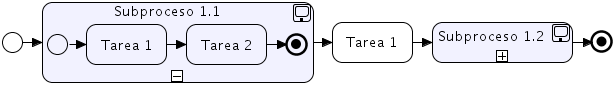
\includegraphics[width=0.8\textwidth]{images/procesos/JerarquiaProcesos2_1}}%
		\caption{Subproceso 1.1.}
		\label{Intro:JerarquiaProcesos2}
		\end{figure}

	\item{\bf Nombre del proceso}. Estará dado por el nombre que presente el subproceso o actividad en el diagrama BPMN.
\end{itemize}

\noindent Por ejemplo:
	\begin{center}
		{\bf PP-A 1.5.1 Pago SPEI}
	\end{center}

\noindent Significa que es el subproceso \textbf{PP-} de Admisión \textbf{A} número \textbf{5} que contiene el subroceso \textbf{1} llamado \textbf{Pago SPEI}.

%---------------------------------------------------------
\subsection{Elementos de un subproceso}

Un {\bf elemento} del subproceso es un atributo utilizado para describir las características de los subprocesos. Los atributos ayudan a entender la funcionalidad e interacción de un subproceso con otro (a través de los insumos de entrada y productos de salida).\\

\noindent Los elementos que describen los subprocesos de Admisión son los siguientes:

\begin{itemize}
	\item {\bf Actores:} Lista de los actores que intervienen en el subproceso.
	\item {\bf Objetivo:} Breve descripción del propósito del subproceso.
	\item {\bf Insumos de entrada:} Lista de datos de entrada requeridos durante la ejecución del subproceso.
	\item {\bf Proveedores:} Son las áreas o personas que proveen insumos al subproceso.
	\item {\bf Productos de salida:} Lista de datos de salida que otorga el subproceso al ser ejecutado.
	\item {\bf Cliente:} Áreas o personas que consumen los productos generados por el subproceso.
	\item {\bf Recursos del proceso}: Son los recursos necesarios para llevar a cabo el subproceso.
	\item {\bf Interrelación con otros procesos:} Es la interacción con otros subprocesos internos y/o externos para verificar la apropiada interacción con estos.
\end{itemize}
 % Introducción al contenido del documento

    %---------- Proceso de Admisión
\chapter{Procesos} 

%====================CELULA1=====================================
%Introducir los correspondientes a la GESTIÓN DE EMPLEADOS
		

%------------------------------------------------------------------------------------------------------------------------------------------------


%========================================================
%Macroproceso Gestion de Personal
%========================================================

%========================================================
% Descripción general del proceso
%-----------------------------------------------
\begin{Proceso}{P1.0}{Gestion de Personal} {
  
  %-------------------------------------------
  %Resumen
Macroproceso que lleva a cabo el \cdtRef{Actor:Jefe de Biblioteca}{Jefe de Biblioteca} para poder hacer la peticiónes para el registro,modificaciones y eliminaciones en el sistema de personal de la biblioteca. Para cada actividad hay un subproceso.
 


  %-------------------------------------------
  %Diagrama del proceso

  \noindent La Figura \cdtRefImg{P1.0}{Gestion de Personal} muestra las actividades que se realizan para llevar a cabo el proceso descrito anteriormente.

  \Pfig[0.95]{./procesos/C1/Images/GU1_0-GestionPersonal.png}{P1.0}{Gestion de Personal}

} {P1.0:Gestion de Personal}

  %-------------------------------------------
  %Elementos del proceso

  \UCitem{Actores} { %Actores
    \cdtRef{Actor:Jefe de Biblioteca}{Jefe de Biblioteca}.
  }

  \UCitem{Objetivo} { %Objetivo
    Hacer el registro, la consulta, la actualizacion de datos y eliminacion del personal de la biblioteca.
  }

  \UCitem{Insumos de entrada} { %Insumos de entrada
	 Seleccion de la actividad a realizar.
  }
  
  \UCitem{Proveedores} { %Proveedores
  \begin{UClist}
  		\UCli Direccion de Capital Humano de ESCOM
    	\UCli Biblioteca General del IPN
    \end {UClist}
    
  }

  \UCitem{Productos de salida} { %Productos de salida
    \begin{UClist}
    
      \UCli Depende del subproceso a realizar.
    \end{UClist}
  }

  \UCitem{Cliente} { %Cliente
    \cdtRef{Actor:Jefe de Biblioteca}{Jefe de Biblioteca}
  }

  \UCitem{Mecanismo de medición} { %Mecanismo de medición
    \begin{UClist}
      \UCli Respuesta inmediata
      
    \end{UClist}
  }


\end{Proceso}

%========================================================
%Descripción de tareas
%-----------------------------------------------
\begin{PDescripcion}

  %Actor: Jefe de Bibliotecca
  \Ppaso Jefe de Biblioteca

    \begin{enumerate}

      %Tarea a
      \Ppaso[\itarea] \cdtLabelTask{T1-P1.0:Jefe de Biblioteca}{Registrar Usuario.} Subproceso en el cual el \cdtRef{Actor:Jefe de Biblioteca}{Jefe de Biblioteca} podra realizar el registro de nuevo personal a la biblioteca. 

\Ppaso[\itarea] \cdtLabelTask{T2-P1.0:Jefe de Biblioteca}{Modificar Usuario.} Subproceso en el cual el \cdtRef{Actor:Jefe de Biblioteca}{Jefe de Biblioteca} podra actualizar los datos del personal.

\Ppaso[\itarea] \cdtLabelTask{T3-P1.0:Jefe de Biblioteca}{Eliminar Usuario.} Subproceso en el cual el \cdtRef{Actor:Jefe de Biblioteca}{Jefe de Biblioteca} podra dar de baja de las funciones de la biblioteca al personal indicado.
	

    \end{enumerate}
    
    
\end{PDescripcion}


%------------------------------------------------------------------------------------------------------------------------------------------------
	
		

%------------------------------------------------------------------------------------------------------------------------------------------------


%========================================================
%Proceso Registrar Personal
%========================================================

%========================================================
% Descripción general del proceso
%-----------------------------------------------
\begin{Proceso}{P1.1}{Registrar Personal} {
  
  %-------------------------------------------
  %Resumen
Proceso que lleva a cabo el \cdtRef{Actor:Jefe de Biblioteca}{Jefe de Biblioteca} para poder hacer la petición y el registro de
nuevo personal.

De manera más especifica este proceso, realiza una petición a la biblioteca general solicitando más personal como pueden ser un nuevo \cdtRef{Actor:Bibliotecario}{Bibliotecario} o un nuevo \cdtRef{Actor:Personal de Procesos Tecnicos}{Personal de Procesos Tecnicos}.
La biblioteca general regresa una respuesta que puede ser afirmativa o negativa.

En caso de que la solicitud haya sido aceptada, la Dirección de capital humano envía los datos del
nuevo personal. Tales datos son el nombre completo, la cedula profesional y el rol a desempeñar
dentro de la biblioteca.
  


  %-------------------------------------------
  %Diagrama del proceso

  \noindent La Figura \cdtRefImg{P1.1}{Registrar Personal} muestra las actividades que se realizan para llevar a cabo el proceso descrito anteriormente.

  \Pfig[0.95]{./procesos/C1/Images/GU1_1-RegistrarPersonal.png}{P1.1}{Registrar Personal}

} {P1.1:Registrar Personal}

  %-------------------------------------------
  %Elementos del proceso

  \UCitem{Actores} { %Actores
    \cdtRef{Actor:Jefe de Biblioteca}{Jefe de Biblioteca}.
  }

  \UCitem{Objetivo} { %Objetivo
    Hacer el registro del nuevo personal, para que este tenga privilegios según sea su rol en la biblioteca.
  }

  \UCitem{Insumos de entrada} { %Insumos de entrada
  	\begin{UClist}
  		\UCli Datos del Formulario \cdtIdRef{F1.1}{Registrar Personal}.
    \end {UClist}
  }
  
  \UCitem{Proveedores} { %Proveedores
    Direccion de Capital Humano de ESCOM
  }

  \UCitem{Productos de salida} { %Productos de salida
    \begin{UClist}
    
      \UCli Tabla generada con los datos correspondientes del \cdtRef{Actor:Bibliotecario}{Bibliotecario} o \cdtRef{Actor:Personal de Procesos Tecnicos}{Personal de Procesos Tecnicos} y su Estado en el sistema.
      \UCli   Notificación \cdtIdRef{MSJ1.1}{Operación exitosa}.
    \end{UClist}
  }

  \UCitem{Cliente} { %Cliente
    \cdtRef{Actor:Jefe de Biblioteca}{Jefe de Biblioteca}
  }

  \UCitem{Mecanismo de medición} { %Mecanismo de medición
    \begin{UClist}
      \UCli Respuesta inmediata
      
    \end{UClist}
  }
  \UCitem{Interrelación con otros procesos} { %Interrelación con otros procesos
    \cdtIdRef{P1.2}{Modificar Personal}
}


\end{Proceso}

%========================================================
%Descripción de tareas
%-----------------------------------------------
\begin{PDescripcion}

  %Actor: Jefe de Bibliotecca
  \Ppaso Jefe de Biblioteca

    \begin{enumerate}

      %Tarea a
      \Ppaso[\itarea] \cdtLabelTask{T1-P1.1:Jefe de Biblioteca}{Solicitud de nuevo personal.}Un administrativo genera una solicitud de personal a biblioteca general, esta puede ser aceptada o rechazada. En caso de rechazo finaliza el proceso, por último si la solicitud es aceptada se puede proceder a la siguiente tarea. 
      %Condiciones
  \begin{itemize}
    %Condición
    \item \cdtIdRef{C1.1}{Autorizacion de registro} el sistema pasa a la tarea \cdtRefTask{T2-P1.1:Jefe de Biblioteca}{Registro de personal.}
  \end{itemize}

\Ppaso[\itarea] \cdtLabelTask{T2-P1.1:Jefe de Biblioteca}{Registro de personal.} El administrativo recibe un documento donde se especifican los datos del nuevo personal como son nombre completo, cedula profesional y finalmente se asigna el rol que desempeñaran dentro de la biblioteca.

	\begin{itemize}
    %Condición
    \item \cdtIdRef{C1.2}{Duplicidad de personal} el sistema pasa a verificar la tarea \cdtRefTask{T2-P1.1:Jefe de Biblioteca}{Registro de personal.}
  \end{itemize}

    \end{enumerate}
    
    
\end{PDescripcion}


%------------------------------------------------------------------------------------------------------------------------------------------------
	
		

%------------------------------------------------------------------------------------------------------------------------------------------------


%========================================================
%Proceso Modificar Personal
%========================================================

%========================================================
% Descripción general del proceso
%-----------------------------------------------
\begin{Proceso}{P1.2}{Modificar Personal} {
  
  %-------------------------------------------
  %Resumen
Proceso que realiza el \cdtRef{Actor:Jefe de Biblioteca}{Jefe de Biblioteca} como primer paso para modificar informacion del personal y para llevarse a cabo se solicita al sistema de biblioteca general, la lista de empleados que necesiten ser modificados o actualizados.
Si existen empleados en la lista para ser modificados, el sistema primero notificara al \cdtRef{Actor:Jefe de Biblioteca}{Jefe de Biblioteca} para que este reciba la lista con los empleados a modificar, de lo contrario la labor será salir del sistema. En caso de que exista dicha lista, se deberá seleccionar la opción correspondiente al tipo de informacion que desea actualizar, se le mostraran las opciones de modificar datos personales, modificar contraseña y modificar área de biblioteca.
Una vez seleccionando la opción se enviara una notificación de modificación al sistema, para que
este realice la operación y al concluirla en caso de que los datos sean correctos se notificara que la
operación ha sido exitosa, o de lo contrario se enviara un mensaje, avisando que los datos son
incorrectos.
En el supuesto caso de ser incorrectos, una vez recibiendo la notificación, el \cdtRef{Actor:Jefe de Biblioteca}{Jefe de Biblioteca} deberá decidir si quiere corregirlos en ese momento o posteriormente, cuando decida corregir, enviara de nuevo la informacion con los datos correctos y este una vez culminado ese proceso, podrá regresar al menú principal para modificar la informacion del siguiente personal y si ha terminado, podrá salir del sistema.


  %-------------------------------------------
  %Diagrama del proceso

  \noindent La Figura \cdtRefImg{P1.2}{Modificar Personal} muestra las actividades que se realizan para llevar a cabo el proceso descrito anteriormente.

  \Pfig[0.95]{./procesos/C1/Images/GU1_2-ModificarPersonal.png}{P1.2}{Modificar Personal}

} {P1.2:Modificar Personal}

  %-------------------------------------------
  %Elementos del proceso

  \UCitem{Actores} { %Actores
    \cdtRef{Actor:Jefe de Biblioteca}{Jefe de Biblioteca}.
    \cdtRef{Actor:Sistema}{Sistema}.
  }

  \UCitem{Objetivo} { %Objetivo
    Tener los datos actualizados y correctos de cada empleado.
  }

  \UCitem{Insumos de entrada} { %Insumos de entrada
  	\begin{UClist}
  		\UCli Datos del Formulario \cdtIdRef{F1.2}{Modificar Personal}.
    \end {UClist}
  }
  
  \UCitem{Proveedores} { %Proveedores
    Sistema
  }

  \UCitem{Productos de salida} { %Productos de salida
    \begin{UClist}
    	\UCli   Notificación \cdtIdRef{MSJ1.2}{Hay empleados a modificar}.
 		\UCli   Notificación \cdtIdRef{MSJ1.3}{Informacion incorrecta}.
    	\UCli   Notificación \cdtIdRef{MSJ1.4}{Modificacion Exitosa}.
    \end{UClist}
  }

  \UCitem{Cliente} { %Cliente
  	\cdtRef{Actor:Jefe de Biblioteca}{Jefe de Biblioteca}
  }

  \UCitem{Mecanismo de medición} { %Mecanismo de medición
    \begin{UClist}
      \UCli Respuesta inmediata
      
    \end{UClist}
  }
  \UCitem{Interrelación con otros procesos} { %Interrelación con otros procesos
    \cdtIdRef{P1.1}{Registrar Personal}
  }


\end{Proceso}

%========================================================
%Descripción de tareas
%-----------------------------------------------
\begin{PDescripcion}

  %Actor: Jefe de Biblioteca
  \Ppaso Jefe de Biblioteca

    \begin{enumerate}

      %Tarea a
      \Ppaso[\itarea] \cdtLabelTask{T1-P1.2:Jefe de Biblioteca}{Solicita modificar a un empleado.}Para obtener la lista de los empleados que requieren cambios en su informacion es necesario pedirla al Sistema de la Biblioteca General, y una vez que llega la lista se espera el siguiente evento:
      \begin{itemize}
      	\item \cdtIdRef{C1.3}{Autorizacion de Modificacion} el sistema pasa a la tarea \cdtRefTask{T2-P1.2:Jefe de Biblioteca}{Registro de personal.}
		\item Si no hay más que modificar sencillamente saldrá del proceso.
      \end{itemize}

	\Ppaso[\itarea] \cdtLabelTask{T2-P1.2:Jefe de Biblioteca}{Selecciona una opcion.} Una vez obtenida la lista, este debe seleccionar una de las 3 opciones que se le presentan las cuales son:
Modificar Datos Personales, Modificar Contraseña y Modificar área
biblioteca. 
Cuando se seleccione la opción :
\begin{itemize}
\item Se manda notificación NS4 ha sido modificado datos personales.
\item Se manda notificación NS5 ha sido modificada la contraseña.
\item Se manda notificación NS6 ha sido modificada el área de biblioteca.
\end{itemize}

Depende de la opción seleccionada.
\begin{itemize}
\item Se recibe notificación de operación exitosa y se vuelve al menú
principal.
\item Se recibe notificación de datos incorrectos, de ser así se le
preguntara si desea corregir, en caso de seleccionar no se acabara
el proceso y saldrá del sistema. Si acepta corregir se pasara a la
siguiente tarea.
\end{itemize}

\Ppaso[\itarea] \cdtLabelTask{T3-P1.2:Jefe de Biblioteca}{Corrige informacion.} En esta sencillamente se corregirán los datos erróneos, para después enviarlos y así repetir el proceso nuevamente.
	\end{enumerate}
    
    \Ppaso Sistema
    \begin{enumerate}
    	\Ppaso[\itarea] \cdtLabelTask{T1-P1.2:Sistema}{Busca lista de empleados para actualizar informacion.} El sistema deberá recaudar a todo el personal que necesiten un cambio en su informacion, una vez reunida la lista se pasara a la siguiente tarea. Si no hay empleados se notificara al administrador para que este solo salga y aquí se romperá el proceso.
    	\Ppaso[\itarea] \cdtLabelTask{T2-P1.2:Sistema}{Muestra lista de empleados.} Se envía la lista del personal \cdtRef{Actor:Jefe de Biblioteca}{Jefe de Biblioteca} para que este pueda trabajar. Cuando el\cdtRef{Actor:Jefe de Biblioteca}{Jefe de Biblioteca} haya modificado se recibirá una
notificación para actualizar los datos. Y entonces el sistema podrá pasar a la siguiente tarea de lo contrario este se mantendrá en espera de respuesta.
	\Ppaso[\itarea] \cdtLabelTask{T3-P1.2:Sistema}{Realiza operacion.} Se actualizan los datos. Se notifica de operación exitosa cuando la informacion sea la correcta y aquí abra terminado el proceso. Se notifica de informacion incorrecta y espera de nuevo una solicitud de modificación.
    	
    \end{enumerate}
\end{PDescripcion}


%------------------------------------------------------------------------------------------------------------------------------------------------

		

%------------------------------------------------------------------------------------------------------------------------------------------------


%========================================================
%Proceso Eliminar Personal
%========================================================

%========================================================
% Descripción general del proceso
%-----------------------------------------------
\begin{Proceso}{P1.3}{Eliminar Personal} {
  
  %-------------------------------------------
  %Resumen
El proceso inicia cuando el \cdtRef{Actor:Jefe de Biblioteca}{Jefe de Biblioteca} solicita la eliminación de un elemento, después dicha solicitud debe ser enviada y procesada por la biblioteca central del politécnico. Habiendo sido aceptada la solicitud, la biblioteca central genera un reporte que se regresa a la biblioteca local, con el cual elimina al personal por medio de una petición al sistema en la cual se envía el usuario y contraseña del elemento a eliminar.
  


  %-------------------------------------------
  %Diagrama del proceso

  \noindent La Figura \cdtRefImg{P1.3}{Eliminar Personal} muestra las actividades que se realizan para llevar a cabo el proceso descrito anteriormente.

  \Pfig[0.95]{./procesos/C1/Images/GU1_3-EliiminarPersonal.png}{P1.3}{Eliminar Personal}

} {P1.3:Eliminar Personal}

  %-------------------------------------------
  %Elementos del proceso

  \UCitem{Actores} { %Actores
    \cdtRef{Actor:Jefe de Biblioteca}{Jefe de Biblioteca}.
    \cdtRef{Actor:Sistema}{Sistema}.
  }

  \UCitem{Objetivo} { %Objetivo
    Eliminar personal del sistema.
  }

  \UCitem{Insumos de entrada} { %Insumos de entrada
  	\begin{UClist}
  		\UCli Contraseña del \cdtRef{Actor:Jefe de Biblioteca}{Jefe de Biblioteca}.
    \end {UClist}
  }
  
  \UCitem{Proveedores} { %Proveedores
    Biblioteca central.
  }

  \UCitem{Productos de salida} { %Productos de salida
    \begin{UClist}
      \UCli   Notificación \cdtIdRef{MSJ1.5}{Eliminacion exitosa}.
    \end{UClist}
  }

  \UCitem{Cliente} { %Cliente
    \cdtRef{Actor:Jefe de Biblioteca}{Jefe de Biblioteca}
  }

  \UCitem{Mecanismo de medición} { %Mecanismo de medición
    \begin{UClist}
      \UCli Respuesta inmediata
      
    \end{UClist}
  }
  \UCitem{Interrelación con otros procesos} { %Interrelación con otros procesos
    \cdtIdRef{P1.2}{Modificar Personal}

  }

\end{Proceso}

%========================================================
%Descripción de tareas
%-----------------------------------------------
\begin{PDescripcion}

  %Actor: Jefe de Bibliotecca
  \Ppaso Jefe de Biblioteca

    \begin{enumerate}

      %Tarea a
      \Ppaso[\itarea] \cdtLabelTask{T1-P1.3:Jefe de Biblioteca}{Solicitar eliminar empleado.}El \cdtRef{Actor:Jefe de Biblioteca}{Jefe de Biblioteca} solicita a biblioteca central por medio de un documento escrito, la aprobación para la eliminación de un elemento del personal de biblioteca. 

  %Condiciones
  \begin{itemize}
    %Condición
    \item \cdtIdRef{C1.4}{Autorizacion de eliminacion} el sistema pasa a la tarea \cdtRefTask{T2-P1.3:Jefe de Biblioteca}{Registro de personal.}
  \end{itemize}

\Ppaso[\itarea] \cdtLabelTask{T2-P1.3:Jefe de Biblioteca}{Recibe reporte de eliminacion.}El jefe de la biblioteca recibe un reporte con los datos del empleado y la autorización o rechazo de la eliminación del elemento.

\Ppaso[\itarea] \cdtLabelTask{T3-P1.3:Jefe de Biblioteca}{Recibe reporte de eliminacion.}Ingresa el usuario y contraseña del empleado a eliminar dentro del sistema y acepta la eliminación.

    \end{enumerate}
    
  %Actor: biblioteca central
  \Ppaso Biblioteca Central

    \begin{enumerate}

      %Tarea a
      \Ppaso[\itarea] \cdtLabelTask{T1-P1.3:Biblioteca Central}{Recibe Solicitud de eliminacion.}Recibe la petición para la eliminación del empleado y determina si es aprobada
o rechazada según las políticas internas de dicha biblioteca.

\Ppaso[\itarea] \cdtLabelTask{T2-P1.3:Biblioteca Central}{Genera reporte de eliminacion.}Se genera un reporte completo con los datos del empleado y los motivos de eliminación, así como las fechas exactas en las que termina su participación en su labor. El reporte se envía de vuelta al jefe.

    \end{enumerate}    
    
%Actor: Sistema
  \Ppaso Sistema

    \begin{enumerate}

      %Tarea a
      \Ppaso[\itarea] \cdtLabelTask{T1-P1.3:Sistema}{Elimina empleado.}Elimina al empleado del sistema y envía los datos de la eliminación al jefe de biblioteca.  
    
    \end{enumerate} 
        
\end{PDescripcion}


%------------------------------------------------------------------------------------------------------------------------------------------------
	


%====================CELULA2=====================================
%Introducir los correspondientes a la GESTIÓN DE INVENTARIO
		%-----------------------------------------------------------------------------------------------------------------------------------------------
%========================================================
%Proceso Actualizar datos de un Alumno
%========================================================

%========================================================
% Descripción general del proceso
%-----------------------------------------------
\begin{Proceso}{P2.1}{Adquisición de Libros} {
  
  %-------------------------------------------
  %Resumen

  Proceso que realiza el \cdtRef{Actor:Bibliotecario}{Bibliotecario} con la finalidad de obtener nuevos ejemplares de libros que se requieren de acuerdo a las asignaturas de cada academia y sujeto al presupuesto establecido por Recursos Materiales. 
  
  Cada jefe de academia es encargado de ques los profesores de realicen una propuesta de libros para evaluarlas de acuerdo a su nivel de importancia y hacer un selección que es enviada al bibliotecario para que éste último realice el pedido. Al efectuar el pago se espera la entrega, se verifica el pedido y se lleva a cabo el proceso de registro y preparación de los libros para su disponibilidad en biblioteca.
  
  %-------------------------------------------
  %Diagrama del proceso
  \newpage
  \noindent La Figura \cdtRefImg{P2.1}{Adquirir Libros} muestra las actividades que se realizan para llevar a cabo el proceso descrito anteriormente.

  \Pfig[0.85]{./procesos/C2/Images/adquirirLibros.png}{P2.1}{Adquirir Libros}

} {P2.1:Adquirir Libros}

  %-------------------------------------------
  %Elementos del proceso
  \UCitem{Actores} { %Actores
    \cdtRef{Actor:Bibliotecario}{Bibliotecario}
  }

  \UCitem{Objetivo} { %Objetivo
    Obtener nuevos ejemplares de libros para la biblioteca.
  }

  \UCitem{Insumos de entrada} { %Insumos de entrada
  	\begin{UClist}
  		\UCli Datos del Formulario \cdtIdRef{F2.1}{Petición de Libros}. 
     	
    \end {UClist}
  }
  
  \UCitem{Proveedores} { %Proveedores
    \cdtRef{Actor:Bibliotecario}{Bibliotecario}
  }

  \UCitem{Productos de salida} { %Productos de salida
    \begin{UClist}
		\UCli	Actualización de los libros disponibles.
    \end{UClist}
  }

  \UCitem{Cliente} { %Cliente
    \cdtRef{Actor:Bibliotecario}{Bibliotecario}
  }

  \UCitem{Mecanismo de medición} { %Mecanismo de medición
    \begin{UClist}
      \UCli Respuesta inmediata
    \end{UClist}
  }
  \UCitem{Interrelación con otros procesos} { %Interrelación con otros procesos
  }


\end{Proceso}
%========================================================
%Descripción de tareas
%-----------------------------------------------
\begin{PDescripcion}

  \Ppaso Bibliotecario
	\begin{enumerate}
		\Ppaso[\itarea] \cdtLabelTask{T1-P2.1:Bibliotecario}{Recepción de Presupuesto} El \cdtRef{Actor:Bibliotecario}{Bibliotecario} recibe el comunicado de Recursos Materiales sobre el presupuesto para comprar libros e informa a los jefes de académia.
	\end{enumerate}

	\begin{enumerate}
		\Ppaso[\itarea] \cdtLabelTask{T2-P2.1:Bibliotecario}{Recepción de petición de Libros} El \cdtRef{Actor:Bibliotecario}{Bibliotecario} recibe la lista con la petición de libros a pedir y junta en una sola lista.
	\end{enumerate}

	\begin{enumerate}
		\Ppaso[\itarea] \cdtLabelTask{T3-P2.1:Bibliotecario}{Recepción de Libros} El \cdtRef{Actor:Bibliotecario}{Bibliotecario} recibe los ejemplares comprados por Recursos Materiales y verifica la entrega para proceder a la prepraración de los libros.
	\end{enumerate}	
%%		\cdtRefTask{T2-P4.3:Bibliotecario}{Autentificar Lector.}	
\end{PDescripcion}


%------------------------------------------------------------------------------------------------------------------------------------------------



		%-----------------------------------------------------------------------------------------------------------------------------------------------
%========================================================
%Proceso Actualizar datos de un Alumno
%========================================================

%========================================================
% Descripción general del proceso
%-----------------------------------------------
\begin{Proceso}{P2.2}{Cotejar Existencia de Libros} {
  
  %-------------------------------------------
  %Resumen

  Proceso que realiza el \cdtRef{Actor:Bibliotecario}{Bibliotecario} cada semestre con la finalidad de conocer el comparativo de los libros físicos que se tienen en biblioteca con los libros que debería haber de acuerdo al inventario final anterior o de acuerdo a la última entrada de ejemplares.
  
  El \cdtRef{Actor:Bibliotecario}{Bibliotecario} procede a cerrar la biblioteca para limpiar los libros y revisar su estado físico, obtener su código e introducirlo en el sistema donde se crea un formato de inventario con los códigos.  Éste formato se envía al sistema interno del IPN donde se realiza el comparativo y se devuelve el oficio con las diferencias de inventario.
  
  Se identifican los libros que están reportados como faltantes y se verifica si un alumno posee el libro, de ser así se agrega como parte del inventario y en caso contrario se cambia el estado del libro a extraviado.
  
  %-------------------------------------------
  %Diagrama del proceso
  \noindent La Figura \cdtRefImg{P2.2}{Cotejar Existencia de Libros} muestra las actividades que se realizan para llevar a cabo el proceso descrito anteriormente.

  \Pfig[1.0]{./procesos/C2/Images/cotejarExistencias.png}{P2.2}{Cotejar Existencia de Libros}

} {P2.2:Cotejar Existencia de Libros}

  %-------------------------------------------
  %Elementos del proceso
  \UCitem{Actores} { %Actores
    \cdtRef{Actor:Bibliotecario}{Bibliotecario} y 
    \cdtRef{Actor:Lector}{Lector}
  }

  \UCitem{Objetivo} { %Objetivo
    Comparar la existencia de libros en biblioteca con el inventario anterior.
  }

  \UCitem{Insumos de entrada} { %Insumos de entrada
  	\begin{UClist}
  		\UCli Identificadores de libros proporcionados por el \cdtRef{Actor:Bibliotecario}{Bibliotecario} en el formulario \cdtIdRef{F2.2}{Agregar Libros a Inventario}. 
     	
    \end {UClist}
  }
  
  \UCitem{Proveedores} { %Proveedores
    \cdtRef{Actor:Bibliotecario}{Bibliotecario}
  }

  \UCitem{Productos de salida} { %Productos de salida
    \begin{UClist}
		\UCli	Actualización del estado de los libros.
    \end{UClist}
  }

  \UCitem{Cliente} { %Cliente
    \cdtRef{Actor:Bibliotecario}{Bibliotecario}
  }

  \UCitem{Mecanismo de medición} { %Mecanismo de medición
    \begin{UClist}
      \UCli Respuesta inmediata
    \end{UClist}
  }
  \UCitem{Interrelación con otros procesos} { %Interrelación con otros procesos
  	    \begin{UClist}
  	    	\UCli Préstamo
  	    \end{UClist}
  }


\end{Proceso}
%========================================================
%Descripción de tareas
%-----------------------------------------------
\begin{PDescripcion}

  \Ppaso Bibliotecario
	\begin{enumerate}
		\Ppaso[\itarea] \cdtLabelTask{T1-P2.2:Bibliotecario}{Entradas de Identificadores} El \cdtRef{Actor:Bibliotecario}{Bibliotecario} cierra la biblioteca y comienza el proceso de inventario introduciendo los identificadores de los libros en el sistema.
		
		\Ppaso[\itarea] \cdtLabelTask{T2-P2.2:Bibliotecario}{Envío y Recepción de Comparativo} El \cdtRef{Actor:Bibliotecario}{Bibliotecario} envía al servidor interno del instituto el reporte de los libros de los que se han introducido su identificador. Recibe como respuesta la lista de libros faltantes.
		
		\Ppaso[\itarea] \cdtLabelTask{T3-P2.2:Bibliotecario}{Identificación de Libros Faltantes} El \cdtRef{Actor:Bibliotecario}{Bibliotecario} consulta a préstamos los libros faltantes. Si los posee un alumno el libro se agrega al inventario, de lo contrario se reporta como perdido.
	\end{enumerate}
%%		\cdtRefTask{T2-P4.3:Bibliotecario}{Autentificar Lector.}	
\end{PDescripcion}


%------------------------------------------------------------------------------------------------------------------------------------------------



		%-----------------------------------------------------------------------------------------------------------------------------------------------
%========================================================
%Proceso Actualizar datos de un Alumno
%========================================================

%========================================================
% Descripción general del proceso
%-----------------------------------------------
\begin{Proceso}{P2.3}{Cotejar Existencia de Equipo} {
  
  %-------------------------------------------
  %Resumen

  Proceso que realiza el \cdtRef{Actor:Bibliotecario}{Bibliotecario} cada 20 de Diciembre con la finalidad de conocer el comparativo del equipo de cómputo, dedicado a préstamo, que se tiene en biblioteca  con el que debería haber de acuerdo al inventario final anterior o de acuerdo a la última entrada de equipo.
  
  El \cdtRef{Actor:Bibliotecario}{Bibliotecario} procede a cerrar la biblioteca para limpiar los equipos y obtener su código e introducirlo en el sistema donde se crea un formato de inventario con los códigos.  Éste formato se envía al sistema interno del IPN donde se realiza el comparativo y se devuelve el oficio con las diferencias de inventario.
  
  Se identifican los equipos que están reportados como faltantes y se verifica si está en almacén, de ser así se agrega como parte del inventario y en caso contrario se cambia el estado del equipo a extraviado.
  
  %-------------------------------------------
  %Diagrama del proceso
  \noindent La Figura \cdtRefImg{P2.3}{Cotejar Existencia de Equipo} muestra las actividades que se realizan para llevar a cabo el proceso descrito anteriormente.

  \Pfig[1.0]{./procesos/C2/Images/cotejarExistenciasEquipo.png}{P2.3}{Cotejar Existencia de Equipo}

} {P2.3:Cotejar Existencia de Equipo}

  %-------------------------------------------
  %Elementos del proceso
  \UCitem{Actores} { %Actores
    \cdtRef{Actor:Bibliotecario}{Bibliotecario} y 
    \cdtRef{Actor:Lector}{Lector}
  }

  \UCitem{Objetivo} { %Objetivo
    Comparar la existencia del equipo de cómputo en biblioteca con el inventario anterior.
  }

  \UCitem{Insumos de entrada} { %Insumos de entrada
  	\begin{UClist}
  		\UCli Identificadores del equipo de cómputo proporcionados por el \cdtRef{Actor:Bibliotecario}{Bibliotecario} en el formulario \cdtIdRef{F2.3}{Agregar Equipo de Cómputo a Inventario}. 
    \end {UClist}
  }
  
  \UCitem{Proveedores} { %Proveedores
    \cdtRef{Actor:Bibliotecario}{Bibliotecario}
  }

  \UCitem{Productos de salida} { %Productos de salida
    \begin{UClist}
		\UCli	Actualización del estado del equipo de cómputo.
    \end{UClist}
  }

  \UCitem{Cliente} { %Cliente
    \cdtRef{Actor:Bibliotecario}{Bibliotecario}
  }

  \UCitem{Mecanismo de medición} { %Mecanismo de medición
    \begin{UClist}
      \UCli Respuesta inmediata
    \end{UClist}
  }
  \UCitem{Interrelación con otros procesos} { %Interrelación con otros procesos
  }


\end{Proceso}
%========================================================
%Descripción de tareas
%-----------------------------------------------
\begin{PDescripcion}

  \Ppaso Bibliotecario
	\begin{enumerate}
		\Ppaso[\itarea] \cdtLabelTask{T1-P2.2:Bibliotecario}{Entradas de Identificadores} El \cdtRef{Actor:Bibliotecario}{Bibliotecario} cierra la biblioteca y comienza el proceso de inventario introduciendo los identificadores del equipo de cómputo en el sistema.
		
		\Ppaso[\itarea] \cdtLabelTask{T2-P2.2:Bibliotecario}{Envío y Recepción de Comparativo} El \cdtRef{Actor:Bibliotecario}{Bibliotecario} envía al servidor interno del instituto el reporte de los equipos de los que se han introducido su identificador. Recibe como respuesta la lista de equipos faltantes.
		
		\Ppaso[\itarea] \cdtLabelTask{T3-P2.2:Bibliotecario}{Identificación de Equipos Faltantes} El \cdtRef{Actor:Bibliotecario}{Bibliotecario} consulta a almacen los equipos faltantes. Si se encuentran se agrega al inventario, de lo contrario se reporta como perdido.
	\end{enumerate}
%%		\cdtRefTask{T2-P4.3:Bibliotecario}{Autentificar Lector.}	
\end{PDescripcion}


%------------------------------------------------------------------------------------------------------------------------------------------------


	
		%-----------------------------------------------------------------------------------------------------------------------------------------------
%========================================================
%Proceso Actualizar datos de un Alumno
%========================================================

%========================================================
% Descripción general del proceso
%-----------------------------------------------
\begin{Proceso}{P2.4}{Descartar libros } {
  
  %-------------------------------------------
  %Resumen

  Proceso que realiza el \cdtRef{Actor:Bibliotecario}{Bibliotecario} con la finalidad de llevar a cabo el descarte de libros por diversas razones al final de su vida util o por defectos que conlleva a dar de baja un libro del inventario.
  Se reúnen los libros que se encuentren en algún estado de los siguientes:
  -obsolescencia.
  -falta de uso.
  -contaminación y/o mutilación.
Despues se informa a la oficina de recursos materiales del ipn el problema de libros con eso recibe un formato de la oficina de recursos el cual contiene nombre título autores edición y motivo de descarte por cada isbn se necesita llenar el formato anterior.
Despues los libros se guardan en una caja y se envían junto con su formato pegado en la caja a recursos materiales del ipn con ello la biblioteca  es informada mediante un acuse de recibo que los libros han sido entregados satisfactoriamente.



  %-------------------------------------------
  %Diagrama del proceso

  \noindent La Figura \cdtRefImg{P2.4}{Descartar libros} muestra las actividades que se realizan para llevar a cabo el proceso descrito anteriormente.

  \Pfig[0.95]{./procesos/C2/Images/GU4_6Descartar.png}{P4.6}{Descartar libros}
\Pfig[0.95]{./procesos/Ejemplo/Images/PA2_1-SolicitudDeCuenta.png}{P0.1}{Solicitud de cuenta}

} {P4.6:Realizar Descarte de libros}

  %-------------------------------------------
  %Elementos del proceso

  \UCitem{Actores} { %Actores
    \cdtRef{Actor:Bibliotecario}{Bibliotecario} .
  }

  \UCitem{Objetivo} { %Objetivo
	Descartar un libro para darlo de baja del sistema en el inventario.
  }

  \UCitem{Insumos de entrada} { %Insumos de entrada
  	\begin{UClist}
  		\UCli Recuperacion de los libros para descartar dependiendo de la informacion de el estado de los libros.
     	
    \end {UClist}
  }
  
  \UCitem{Proveedores} { %Proveedores
    Sistema
  }

  \UCitem{Productos de salida} { %Productos de salida
    \begin{UClist}
    
      \UCli Acuse de recibido.
      \UCli Libros dados de baja del sistema.
  
    \end{UClist}
  }

  \UCitem{Cliente} { %Cliente
    \cdtRef{Actor:Bibliotecario}{Bibliotecario}
  }

  \UCitem{Mecanismo de medición} { %Mecanismo de medición
  
  }
  \UCitem{Interrelación con otros procesos} { %Interrelación con otros procesos
  }


\end{Proceso}

%========================================================
%Descripción de tareas
%-----------------------------------------------
\begin{PDescripcion}

  %Actor: Aspirante
  \Ppaso Encargado de biblioteca

    \begin{enumerate}

      %Tarea a
      \Ppaso[\itarea] \cdtLabelTask{T1-P4.6:Encargado}{Solicitar descarte de libros.}El encargado solicita iniciar el descarte de libros.
	

    \end{enumerate}
    
    
      %Actor: SAEV2.0
  \Ppaso Bibliotecario 

    \begin{enumerate}

      %Tarea a
      \Ppaso[\itarea] \cdtLabelTask{T1-P4.3:Bibliotecario}{.}Se revisa los estados de los libros que se pueden descartar por obsolescencia, falta de uso, contaminación y/o mutilación.

      %Tarea b
      \Ppaso[\itarea] \cdtLabelTask{T2-P4.3:Bibliotecario}{.}se reúnen los libros que se encuentren en algún estado anterior o que reúnan alguna de las características mencionadas anteriormente.
      
      %Tarea c
      \Ppaso[\itarea] \cdtLabelTask{T3-P4.3:Bibliotecario}{.}se informa a la oficina de recursos materiales del ipn el problema de libros.

      %Tarea d
      \Ppaso[\itarea] \cdtLabelTask{T4-P4.3:Bibliotecario}{.}se recibe un formato de la oficina de recursos el cual contiene nombre título autores edición y motivo de descarte.
      
      
      %Tarea e
      \Ppaso[\itarea] \cdtLabelTask{T5-P4.3:Bibliotecario}{.}los libros se guardaran en una caja y se envían junto con su formato pegado en la caja a recursos materiales del ipn.

      %Tarea f
      \Ppaso[\itarea] \cdtLabelTask{T3-P4.3:Bibliotecario}{.}el bibliotecario  es informado mediante un acuse de recibo que los libros han sido entregados satisfactoriamente.
      
          \end{enumerate}

\end{PDescripcion}


%------------------------------------------------------------------------------------------------------------------------------------------------
	
		%%========================================================
%Proceso
%========================================================

%========================================================
% Descripción general del proceso
%-----------------------------------------------
\begin{Proceso}{P0.1}{Reposición de libro} {
  
  %-------------------------------------------
  %Resumen

  Proceso que realiza el \cdtRef{Actor:Aspirante}{Aspirante} cuando un libro que le ha sido prestado previamente está perdido.
  
  Al darse esta situación, el \cdtRef{Actor:SAEV2.0}{SAEV2.0} cancela el privilegio de préstamo al \cdtRef{Actor:Aspirante}{Aspirante} , etiqueta el libro en cuestión como perdido y envía una notificación de prórroga al \cdtRef{Actor:Aspirante}{Aspirante} para poder recuperar el libro, de ser así el proceso termina, de no ser así, el \cdtRef{Actor:Aspirante}{Aspirante} tiene dos opciones, el reemplazo físico del libro en cuestión o bien, el pago del precio del libro, en caso de que decida reemplazar el libro, el \cdtRef{Actor:SAEV2.0}{SAEV2.0} quita la etiqueta de perdido del libro en cuestion, si en cambio desea pagar el precio del libro, entonces el \cdtRef{Actor:SAEV2.0}{SAEV2.0} quita la etiqueta de perdido del libro y además lo pone en una lista de libros a adquirir.


  %-------------------------------------------
  %Diagrama del proceso

  \noindent La Figura \cdtRefImg{P0.1}{Solicitud de cuenta} muestra las actividades que se realizan para llevar a cabo el proceso descrito anteriormente.

  \Pfig[0.95]{.Biblioteca3CM2/Documentacion/DocumentoProcesos/images/procesoreposiciondelibros.png}{P0.1}{Solicitud de cuenta}

} {P0.1:Cuenta}

  %-------------------------------------------
  %Elementos del proceso

  \UCitem{Actores} { %Actores
    \cdtRef{Actor:Aspirante}{Aspirante} y \cdtRef{Actor:SAEV2.0}{SAEV2.0}.
  }

  \UCitem{Objetivo} { %Objetivo
    Que el \cdtRef{Actor:Aspirante}{Aspirante} realice la reposición de un libro perdido.
  }

  \UCitem{Insumos de entrada} { %Insumos de entrada
  	\begin{UClist}
  		\UCli N A
    \end {UClist}
  }
  
  \UCitem{Proveedores} { %Proveedores
    \cdtRef{Actor:Aspirante}{Aspirante}
  }

  \UCitem{Productos de salida} { %Productos de salida
    \begin{UClist}
      \UCli Notificación
    \end{UClist}
  }

  \UCitem{Cliente} { %Cliente
    \cdtRef{Actor:Aspirante}{Aspirante}
  }

  \UCitem{Mecanismo de medición} { %Mecanismo de medición
    \begin{UClist}
      \UCli Un día hábil  de asignación PENDIENTE
      \UCli Cuatro días  hábiles de evaluación
    \end{UClist}
  }
  \UCitem{Interrelación con otros procesos} { %Interrelación con otros procesos
    \begin{UClist}
      \UCli PENDIENTE
    \end {UClist}
  }


\end{Proceso}

%========================================================
%Descripción de tareas
%-----------------------------------------------
\begin{PDescripcion}

  %Actor: Aspirante
  \Ppaso Aspirante

    \begin{enumerate}

      %Tarea a
      \Ppaso[\itarea] \cdtLabelTask{T1-P0.1:Aspirante}{Reemplazar el libro.} El \cdtRef{Actor:Aspirante}{Aspirante} debe reemplazar el libro perdido con otro que sea exactamente el mismo ISBN y que esté en buenas condiciones.

      %Tarea b
      \Ppaso[\itarea] \cdtLabelTask{T1-P0.1:Aspirante}{Pagar el libro.} El \cdtRef{Actor:Aspirante}{Aspirante} debe pagar el precio exacto del libro.


    \end{enumerate}

  %Actor: SAEV2.0
  \Ppaso SAEV2.0

    \begin{enumerate}

      %Tarea a
      \Ppaso[\itarea] \cdtLabelTask{T1-P0.1:SAEV2.0}{Cancela los privilegios de préstamo.} Le quita al \cdtRef{Actor:Aspirante}{Aspirante} los privilegios para poder pedir un libro prestado.

      %Tarea b
      \Ppaso[\itarea] \cdtLabelTask{T2-P0.1:SAEV2.0}{Etiquetar el libro como perdido} Pone la etiqueta de perdido en el campo de estado de la base de datos de los libros, para que se sepa que este se encuentra fuera de disponibilidad hasta que la reposicion se lleve a cabo, entonces sucede el siguiente evento:
      \begin{itemize}
    %Evento 1
    \item Envía la notificación \cdtIdRef{MSJ0.2}{Usted tiene una prórroga de 3 dias hábiles para devolver el libro, de lo contrario deberá proceder a reemplazarlo}
      \end{itemize}

      %Tarea c
      \Ppaso[\itarea] \cdtLabelTask{T3-P0.1:SAEV2.0}{Quita etiqueta de perdido} Quita la etiqueta de perdido del libro, volviendo esta etiqueta a ser disponible, para que se sepa que el libro está disponible para consulta o préstamo.

      %Tarea d
      \Ppaso[\itarea] \cdtLabelTask{T3-P0.1:SAEV2.0}{Reactiva los privilegios de préstamo} Le otorga al \cdtRef{Actor:Aspirante}{Aspirante} los privilegios para pedir un libro en préstamo.


    \end{enumerate}

\end{PDescripcion}



%====================CELULA3=====================================
%Introducir los correspondientes a la GESTIÓN DE PRÉSTAMOS



%====================CELULA4=====================================
%Introducir los correspondientes a la GESTIÓN DE USUARIOS
		

%------------------------------------------------------------------------------------------------------------------------------------------------


%========================================================
%Proceso Cambiar estado de Alumno
%========================================================

%========================================================
% Descripción general del proceso
%-----------------------------------------------
\begin{Proceso}{P4.1}{Dar de Alta Lector} {
  
  %-------------------------------------------
  %Resumen

Proceso que realiza el \cdtRef{Actor:Lector}{Lector}, con el fin de tener acceso a los prestamos bibliotecarios, y tenga el derecho de estar monitoreado su perfil y así visualizar el \cdtRef{Actor:Bibliotecario}{Bibliotecario} en qué estado se encuentra el \cdtRef{Actor:Lector}{Lector}.
  
  
Para poder tener un Registro en la Biblioteca, el \cdtRef{Actor:Lector}{Lector} deberá de contar con los requisitos del formulario que pide dicho organismo para validar los datos, y que haga valer la RN4.1 Lector Inscrito en el instituto y la RN4.3 Formato 4.1 llenado correctamente, ya que al no estar inscrito a la escuela, no podrá formar parte del proceso de registro a la Biblioteca.
  


  %-------------------------------------------
  %Diagrama del proceso

  \noindent La Figura \cdtRefImg{P4.1}{Dar de Alta Lector} muestra las actividades que se realizan para llevar a cabo el proceso descrito anteriormente.

  \Pfig[0.95]{./procesos/C4/Images/GU4_1-DardeAltaLector.jpg}{P4.1}{Dar de Alta Lector}

} {P4.1:Dar de Alta Lector}

  %-------------------------------------------
  %Elementos del proceso

  \UCitem{Actores} { %Actores
    \cdtRef{Actor:Bibliotecario}{Bibliotecario} y \cdtRef{Actor:Lector}{Lector}.
  }

  \UCitem{Objetivo} { %Objetivo
    Validar Datos y generar el registro del \cdtRef{Actor:Lector}, para que este tenga privilegios según el perfil en la biblioteca.
  }

  \UCitem{Insumos de entrada} { %Insumos de entrada
  	\begin{UClist}
  		\UCli Datos del Formulario \cdtIdRef{F4.1}{Dar de alta Lector}.
    \end {UClist}
  }
  
  \UCitem{Proveedores} { %Proveedores
    \cdtRef{Actor:Lector}{Lector}
  }

  \UCitem{Productos de salida} { %Productos de salida
    \begin{UClist}
    
      \UCli Tabla generada con los datos correspondientes del  \cdtRef{Actor:Lector}{Lector} y su Estado en el sistema.
      \UCli   Notificación \cdtIdRef{MSJ4.1}{Lector no registrado}.
      \UCli   Notificación \cdtIdRef{MSJ4.5}{Operación exitosa}.
    \end{UClist}
  }

  \UCitem{Cliente} { %Cliente
    \cdtRef{Actor:Lector}{Lector}
  }

  \UCitem{Mecanismo de medición} { %Mecanismo de medición
    \begin{UClist}
      \UCli Respuesta inmediata
      
    \end{UClist}
  }
  \UCitem{Interrelación con otros procesos} { %Interrelación con otros procesos
    \cdtIdRef{P4.4}{Consultar historial de Lector}
  }


\end{Proceso}

%========================================================
%Descripción de tareas
%-----------------------------------------------
\begin{PDescripcion}

  %Actor: Aspirante
  \Ppaso Lector

    \begin{enumerate}

      %Tarea a
      \Ppaso[\itarea] \cdtLabelTask{T1-P4.1:Lector}{Inscribir al Instituto.}Tendra que inscribirse a la Escuela para que el Bibliotecario pueda generar el registro al organismo y proporcionar los datos correspondientes al \cdtRef{Actor:Bibliotecario}{Bibliotecario} para que este pueda validar la información adquirida y pueda empezar el registro a la Biblioteca. 

\Ppaso[\itarea] \cdtLabelTask{T2-P4.1:Lector}{Completa Datos.} Proporcionará los datos completos, según el Formato 1, de lo contrario termina el proceso.

	

    \end{enumerate}
    
    
      %Actor: SAEV2.0
  \Ppaso Bibliotecario 

    \begin{enumerate}

      %Tarea a
      \Ppaso[\itarea] \cdtLabelTask{T1-P4.1:Bibliotecario}{Validar datos de Lector.} Valida los datos del \cdtRef{Actor:Lector}{Lector} Según el Formato 1 que estén completos y que sea un \cdtRef{Actor:Lector}{Lector} inscrito y/o Registrado a la escuela, si la regla de negocio se cumple pasa a la tarea \cdtRefTask{T2-P4.1:Bibliotecario}{Datos Incompletos.}, donde valida por completo que los datos estén completos, si no cumple con la regla de negocio, termina el proceso. Este notifica al \cdtRef{Actor:Lector}{Lector} que deberá de inscribirse a la escuela.

%referenciar tareas \cdtRefTask{T2-P0.1:SAEV2.0}{Notifica solicitud fuera de periodo de registro.}


      %Tarea b
      \Ppaso[\itarea] \cdtLabelTask{T2-P4.1:Bibliotecario}{Datos Incompletos.} Valida que los datos este completos, si los datos están completos, pasa a la tarea \cdtRefTask{T3-P4.1:Bibliotecario}{Registro.} que registra los datos en el sistema, si no están completos el sistema genera una notificación que mostrara al Bibliotecario que los datos son incompletos, y este le notificara al Lector.
      
      %Tarea c
      \Ppaso[\itarea] \cdtLabelTask{T3-P4.1:Bibliotecario}{Registro.}Registra los datos del Lector en el sistema y genera la Notificación \cdtIdRef{MSJ4.5}{Operación exitosa} para mostrarlo al \cdtRef{Actor:Lector}{Lector}.
     

          \end{enumerate}

\end{PDescripcion}


%------------------------------------------------------------------------------------------------------------------------------------------------
		
		%========================================================
%Proceso
%========================================================

%========================================================
% Descripción general del proceso
%-----------------------------------------------
\begin{Proceso}{P4.2}{Dar de Baja Lector} {
  
  %-------------------------------------------
  %Resumen



  Proceso que realiza el \cdtRef{Actor:Bibliotecario}{Bibliotecario} con el fin de dar de baja a un \cdtRef{Actor:Lector}{Lector} ya sea alumno o docente del sistema siguiendo reglas de negocio que permiten que el usuario sea dado de baja cuando se encuentre libre de adeudos y multas.
  
Como primer paso se tendrá que validar al lector mediante su credencial de manera que se compruebe que este registrado en el sistema.
Si el lector al que se dará de baja tiene adeudos o multas pendientes, el sistema se encargará de notificar al bibliotecario posteriormente se mostraran los adeudos y multas que corresponden al lector.


  Para que proceda la baja, el \cdtRef{Actor:Lector}{Lector} tiene la responsabilidad tanto de pagar sus multas y devolver el material que tiene pendiente, de lo contrario la baja no procederá.
El sistema termina el proceso de dar de baja. 

  %-------------------------------------------
  %Diagrama del proceso

  \noindent La Figura \cdtRefImg{P4.2}{Dar de baja Lector} muestra las actividades que se realizan para llevar a cabo el proceso descrito anteriormente.

  \Pfig[0.95]{./procesos/C4/Images/GU4_2-DarDeBajaLector.png}{P4.2}{Dar de Baja Lector}

} {P4.2:Dar de Baja Lector}

  %-------------------------------------------
  %Elementos del proceso

  \UCitem{Actores} { %Actores
    \cdtRef{Actor:Lector}{Lector} y \cdtRef{Actor:Bibliotecario}{Bibliotecario}.
  }

  \UCitem{Objetivo} { %Objetivo
    Dar de baja a un lector verificando que no tenga adeudos o multas en su historial.
  }

  \UCitem{Insumos de entrada} { %Insumos de entrada
  	\begin{UClist}
  		\UCli Id del Lector
    \end {UClist}
  }
  
  \UCitem{Proveedores} { %Proveedores
    \cdtRef{Actor:Lector}{Lector}
  }

  \UCitem{Productos de salida} { %Productos de salida
    \begin{UClist}
      \UCli Notificación \cdtIdRef{MSJ4.5}{Operación Exitosa}.
      \UCli Notificación \cdtIdRef{MSJ4.1}{Lector No registrado}.
            \UCli Notificación \cdtIdRef{MSJ4.2}{Tienes Adeudos pendientes}.
            \UCli Tabla que contiene las multas pendientes del \cdtRef{Actor:Lector}{Lector}.
\UCli Notificación \cdtIdRef{MSJ4.4}{Tienes Multas pendientes}.            
\UCli Tabla que contiene los adeudos pendientes del \cdtRef{Actor:Lector}{Lector}.

    \end{UClist}
  }

  \UCitem{Cliente} { %Cliente
    \cdtRef{Actor:Lector}{Lector}
  }

  \UCitem{Mecanismo de medición} { %Mecanismo de medición
    \begin{UClist}
      \UCli Respuesta inmediata
    \end{UClist}
  }
  \UCitem{Interrelación con otros procesos} { %Interrelación con otros procesos
    \cdtIdRef{P4.4}{Consulta Historial de lector}
  }


\end{Proceso}

%========================================================
%Descripción de tareas
%-----------------------------------------------
\begin{PDescripcion}

  %Actor: Aspirante
  \Ppaso Lector

    \begin{enumerate}

      %Tarea a
      \Ppaso[\itarea] \cdtLabelTask{T1-P4.2:Lector}{Pagar Multas.}Notifica al lector que tiene multas pendientes y debe pagarlas de lo contrario no se puede dar de baja.
      %Tarea b
      \Ppaso[\itarea] \cdtLabelTask{T2-P4.2:Lector}{Devuelve el material.}Devuelve el material. Notifica al lector que aún tiene devoluciones pendientes y debe devolver el material, de lo contrario la baja no procederá.

    \end{enumerate}

  %Actor: SAEV2.0
  \Ppaso Bibliotecario

    \begin{enumerate}

      %Tarea a
      \Ppaso[\itarea] \cdtLabelTask{T1-P4.2:Bibliotecario}{Validar al Lector.} Para que el sistema pueda validar al lector debe verificar la Regla de negocio \cdtIdRef{C4.4}{Identificación del lector}. Si la regla de negocio se cumple pasa a la tarea \cdtRefTask{T3-P4.2:Bibliotecario}{Dar de baja Lector}, si no se cumple la regla de negocio el sistema pasa a la tarea \cdtRefTask{T2-P4.2:Bibliotecario}{Autenticar Lector}.

%referenciar tareas \cdtRefTask{T2-P0.1:SAEV2.0}{Notifica solicitud fuera de periodo de registro.}


      %Tarea b
      \Ppaso[\itarea] \cdtLabelTask{T2-P4.2:Bibliotecario}{Autenticar Lector.} El sistema autenticará al lector a partir del ID del mismo para comprobar si el lector está registrado de no estar registrado muestra la Notificación \cdtIdRef{MSJ4.1}{Lector No registrado}.
      %Tarea c
      \Ppaso[\itarea] \cdtLabelTask{T3-P4.2:Bibliotecario}{Dar de baja Lector.}Para que el sistema proceda con la baja del Lector deberá verificar las reglas de negocio \cdtIdRef{C4.5}{El lector tiene multas} y \cdtIdRef{C4.6}{El lector tiene adeudos}. Si las reglas de negocio se cumplen se pasa a la tarea \cdtRefTask{T6-P4.2:Bibliotecario}{Dar de baja Lector}, si no se cumple la \cdtIdRef{C4.5}{El lector tiene multas} se pasa a la tarea \cdtRefTask{T4-P4.2:Bibliotecario}{Generar reporte de multa}, si no se cumple la \cdtIdRef{C4.6}{El lector tiene adeudos} se pasa a la tarea \cdtRefTask{T5-P4.2:Bibliotecario}{Generar reporte de adeudo(s)}.

      %Tarea d
      \Ppaso[\itarea] \cdtLabelTask{T4-P4.2:Bibliotecario}{Generar reporte de multa.} El sistema genera la notificación \cdtIdRef{MSJ4.4}{Tienes Multas pendientes} al igual que la tabla indicando las multas que tiene pendientes a pagar para que sean mostrados al lector pasando a la tarea \cdtRefTask{T1-P4.2:Lector}{Pagar multa(s)}. 

      %Tarea e
      \Ppaso[\itarea] \cdtLabelTask{T5-P4.2:Bibliotecario}{Genera reporte de adeudo(s).} El sistema genera la notificación \cdtIdRef{MSJ4.3}{Tienes Adeudos pendientes} al igual que la tabla indicando los adeudos que tiene pendientes a devolver para que sean mostrados al lector pasando a la tarea \cdtRefTask{T2-P4.2:Lector}{Devueve el material}.

      %Tarea f
      \Ppaso[\itarea] \cdtLabelTask{T6-P4.2:Bibliotecario}{Dar de baja Lector.} El sistema dará de baja al lector y mostrará la notificación \cdtIdRef{MSJ4.5}{Operación Exitosa}.

    \end{enumerate}

\end{PDescripcion}

		%-----------------------------------------------------------------------------------------------------------------------------------------------
%========================================================
%Proceso Actualizar datos de un Alumno
%========================================================

%========================================================
% Descripción general del proceso
%-----------------------------------------------
\begin{Proceso}{P4.3}{Actualizar datos de Lector} {
  
  %-------------------------------------------
  %Resumen

  Proceso que realiza el \cdtRef{Actor:Bibliotecario}{Bibliotecario} con la finalidad tener actualizados los datos del \cdtRef{Actor:Lector}{Lector} cada periodo escolar al inicio del semestre y de esta forma poder continuar con el prestamo de libros de la biblioteca.
  
  En \cdtRef{Actor:Lector}{Lector} solicita la actualización de datos correspondientes en la biblioteca, verifican su registro  solicitando la credencial del instituto y validan si esta inscrito en el sistema de la biblioteca de lo contrario se le notifica que debe realizar el registro. 
  Una vez que la información es enviada correctamente, el  \cdtRef{Actor:Bibliotecario}{Bibliotecario} proporciona un formato para el {Actor:Lector}{Lector} que debe completar correctamente y el {Actor:Bibliotecario}{Bibliotecario} debe asegurarse  que sea un formato valido para proceder a la actualización.   


  %-------------------------------------------
  %Diagrama del proceso

  \noindent La Figura \cdtRefImg{P4.3}{Actualizar datos de Lector} muestra las actividades que se realizan para llevar a cabo el proceso descrito anteriormente.

  \Pfig[0.95]{./procesos/C4/Images/GU4_3-ActualizarLector.png}{P4.3}{Actualizar datos de Lector}

} {P4.3:Actualizar datos de Lector}

  %-------------------------------------------
  %Elementos del proceso

  \UCitem{Actores} { %Actores
    \cdtRef{Actor:Bibliotecario}{Bibliotecario} y \cdtRef{Actor:Letor}{Lector}.
  }

  \UCitem{Objetivo} { %Objetivo
    Actualizar y modificar los  datos de un \cdtRef{Actor:Letor}{Lector}.
  }

  \UCitem{Insumos de entrada} { %Insumos de entrada
  	\begin{UClist}
  		\UCli Datos del Formulario \cdtIdRef{F4.2}{Actualizar Lector}. 
     	
    \end {UClist}
  }
  
  \UCitem{Proveedores} { %Proveedores
    \cdtRef{Actor:Lector}{Lector}
  }

  \UCitem{Productos de salida} { %Productos de salida
    \begin{UClist}
    
      \UCli Tabla actualizada de datos del Alumno.
      \UCli   Notificación \cdtIdRef{MSJ4.5}{Operacion Exitosa}.
       \UCli   Notificación \cdtIdRef{MSJ4.1}{Lector no registrado}.
       \UCli   Notificación \cdtIdRef{MSJ4.7}{Inscribete}.
    \end{UClist}
  }

  \UCitem{Cliente} { %Cliente
    \cdtRef{Actor:Lector}{Lector}
  }

  \UCitem{Mecanismo de medición} { %Mecanismo de medición
    \begin{UClist}
      \UCli Respuesta inmediata
      
    \end{UClist}
  }
  \UCitem{Interrelación con otros procesos} { %Interrelación con otros procesos
  }


\end{Proceso}

%========================================================
%Descripción de tareas
%-----------------------------------------------
\begin{PDescripcion}

  %Actor: Aspirante
  \Ppaso Lector

    \begin{enumerate}

      %Tarea a
      \Ppaso[\itarea] \cdtLabelTask{T1-P4.3:Lector}{Corrige el formato 4.2.} Proporcionará los datos correctos, según el Formato 4.2, de lo contrario termina el proceso.
	

    \end{enumerate}
    
    
      %Actor: SAEV2.0
  \Ppaso Bibliotecario 

    \begin{enumerate}

      %Tarea a
      \Ppaso[\itarea] \cdtLabelTask{T1-P4.3:Bibliotecario}{Validar Lector.} El \cdtRef{Actor:Bibliotecario}{Bibliotecario} solicita la credencial del instituto del \cdtRef{Actor:Lector}{Lector} interesado y el sistema debe verificar la regla de negocio \cdtIdRef{C4.4}{Identificacion del Lector}, si la regla de negocio no se cumple pasa la tarea \cdtRefTask{T2-P4.3:Bibliotecario}{Autentificar Lector.} de lo contrario pasa a la tarea \cdtRefTask{T3-P4.3:Bibliotecario}{Lector no esta inscrito en el instituo.}.


      %Tarea b
      \Ppaso[\itarea] \cdtLabelTask{T2-P4.3:Bibliotecario}{Autentificar Lector.}Muestra la Notificación \cdtIdRef{MSJ4.7}{Inscribete}
      
      %Tarea c
      \Ppaso[\itarea] \cdtLabelTask{T3-P4.3:Bibliotecario}{Lector no esta inscrito en el instituto } Muestra mensaje de nostificación \cdtIdRef{MSJ4.1}{Lector no registrado}.
      .
    %Tarea d
      \Ppaso[\itarea] \cdtLabelTask{T4-P4.3:Bibliotecario}{Actualizar datos del Lector.} El Bibliotecario entrega el formato F4.1 al \cdtRef{Actor:Lector}{Lector} donde se valida la regla de negocio \cdtIdRef{C4.3}{Formato Llenado correctamente},si no se cumple pasa a la tarea \cdtRefTask{T1-P4.3:Lector}{Corrige el formato 4.2.}, pero si se cumple la regla de negocios pasa a la tarea \cdtRefTask{T5-P4.3:Bibliotecario}{Actualizar datos.}
      
      
      %Tarea e
      \Ppaso[\itarea] \cdtLabelTask{T5-P4.3:Bibliotecario}{Actualizar datos.} El \cdtRef{Actor:Bibliotecario}{Bibliotecario} cambia en el sistema los datos del \cdtRef{Actor:Lector}{Lector} donde se notifica que los datos estan actualizados  \cdtIdRef{MSJ4.5}{Operacion Exitosa}.

      
          \end{enumerate}

\end{PDescripcion}


%------------------------------------------------------------------------------------------------------------------------------------------------



		%========================================================
%Proceso
%========================================================

%========================================================
% Descripción general del proceso
%-----------------------------------------------
\begin{Proceso}{P4.4}{Consultar historial de Lector} {
  
  %-------------------------------------------
  %Resumen

  Proceso que realiza el \cdtRef{Actor:Lector}{Lector} desde su perfil con el fin de consultar y visualizar los datos de su historial en el cual se visualizarán los adeudos y/o multas que tenga el \cdtRef{Actor:Lector}{Lector}.
  
Si el \cdtRef{Actor:Lector}{Lector} está registrado en el sistema podrá iniciar Sesióon y tenerun perfil propio desde el cual el \cdtRef{Actor:Lector}{Lector} podrá consultar su historial.
Cuando procede la consulta el sistema generará diferentes tablas presentando los Adeudos, en otra tabla las multas y el estado del \cdtRef{Actor:Lector}{Lector}(activo o inactivo)
El sistema termina el proceso de la consulta 


  %-------------------------------------------
  %Diagrama del proceso

  \noindent La Figura \cdtRefImg{P4.4}{Consulta historial de lector} muestra las actividades que se realizan para llevar a cabo el proceso descrito anteriormente.

  \Pfig[0.95]{./procesos/C4/Images/GU4_4-CosultaLector.png}{P4.4}{Consulta historial de Lector}

} {P4.4:Consulta historial de lector}

  %-------------------------------------------
  %Elementos del proceso

  \UCitem{Actores} { %Actores
    \cdtRef{Actor:Lector}{Lector} y \cdtRef{Actor:PGU}{PGU}
  }

  \UCitem{Objetivo} { %Objetivo
    Consultar el historial de Adeudos y Multas de igual manera el estado de un usuario desde su perfil mostrando los datos en en una tabla.
  }

  \UCitem{Insumos de entrada} { %Insumos de entrada
  	\begin{UClist}
  		\UCli Clic en el Botón consultar Historial
    \end {UClist}
  }
  
  \UCitem{Proveedores} { %Proveedores
    \cdtRef{Actor:Lector}{Lector}
  }

  \UCitem{Productos de salida} { %Productos de salida
    \begin{UClist}
      \UCli Tabla generada mostrando las multas del \cdtRef{Actor:Lector}{Lector}
      \UCli Tabla generada mostrando los adeudos del \cdtRef{Actor:Lector}{Lector}
      \UCli Notificación \cdtIdRef{MSJ4.6}{El lector aun no tiene historial}.
    \end{UClist}
  }

  \UCitem{Cliente} { %Cliente
    \cdtRef{Actor:Lector}{Lector}
  }

  \UCitem{Mecanismo de medición} { %Mecanismo de medición
    \begin{UClist}
      \UCli Respuesta inmediata 
    \end{UClist}
  }
  \UCitem{Interrelación con otros procesos} { %Interrelación con otros procesos
    \cdtIdRef{P4.1}{Dar de baja usuario}
  }


\end{Proceso}

%========================================================
%Descripción de tareas
%-----------------------------------------------
\begin{PDescripcion}

  %Actor: Aspirante
  \Ppaso Lector 

    \begin{enumerate}

      %Tarea a
      \Ppaso[\itarea] \cdtLabelTask{T1-P0.1:Lector}{Clic en consultar historial.} Una vez iniciada sesión el \cdtRef{Actor:Lector}{Lector} dará clic en el botón de consultar historial desde su perfil.
      
            \Ppaso[\itarea] \cdtLabelTask{T2-P4.5:Lector}{No tiene historial.} Se el mostrará la Notificación \cdtIdRef{MSJ4.6}{El lector aun no tiene historial.} 
            
            \Ppaso[\itarea] \cdtLabelTask{T3-P4.5:Lector}{Historial del Lector.} Se le mostrará la tabla del historial.              
            
    \end{enumerate}

  %Actor: SAEV2.0
  \Ppaso PGU
%\cdtRefTask{T2-P0.1:SAEV2.0}{Notifica solicitud fuera de periodo de registro.}
    \begin{enumerate}

      %Tarea a
      \Ppaso[\itarea] \cdtLabelTask{T1-P4.4:PGU}{Verificar Existencia} Para que el sistema pueda consultar y visualizar la información de el \cdtRef{Actor:Lector}{Lector} este debe verificar si el     \cdtRef{Actor:Lector}{Lector} tiene un historial de adeudos o multas de ser asi se pasa a la tarea \cdtRefTask{T2-P4.4:PGU}{Genera tabla con la información del Lector.}, de lo contrario pasa a la tarea \cdtRefTask{T3-P4.4:PGU}{Genera mensaje de inexistencia de historial.}

      %Tarea b
      \Ppaso[\itarea] \cdtLabelTask{T2-P4.4:PGU}{Genera tabla con la información del usuario.} El sistema genera una tabla con la información de los adeudos o multas asociadas al \cdtRef{Actor:Lector}{Lector} para que sea mostrada pasando a la tarea \cdtRefTask{T3-P4.5:Lector}{Información del Lector.}

      %Tarea c
      \Ppaso[\itarea] \cdtLabelTask{T3-P4.4:PGU}{Genera mensaje de inexistencia de historial.} El sistema genera el mensaje de Notificación \cdtIdRef{MSJ4.6}{El lector aun no tiene historial} para que sea mostrado al \cdtRef{Actor:Lector}{Lector} pasando a la tarea \cdtRefTask{T2-P4.5:Lector}{No tiene historial.}

      
    \end{enumerate}

\end{PDescripcion}

		 %Consultar Usuario


%====================CELULA5=====================================
%Introducir los correspondientes a la GESTIÓN DE CREDENCIALES
		%========================================================
%Proceso
%========================================================

%========================================================
% Descripción general del proceso
%-----------------------------------------------
\begin{Proceso}{P5.1}{Gestion de credenciales} {
  
  %-------------------------------------------
  %Resumen

  Proceso que se encarga de la gestión de credenciales, en donde se genera las credenciales para lectores \cdtRef{Actor:Estudiante}{Estudiante} y \cdtRef{Actor:Profesor}{Profesor}. Además de renovar la fecha de vigencia de las credenciales para poder seguir haciendo uso de esta.

  %-------------------------------------------
  %Diagrama del proceso

  \noindent La Figura \cdtRefImg{P5.1}{Gestion de Credenciales} muestra las actividades que se realizan para llevar a cabo el proceso descrito anteriormente.

  \Pfig[0.95]{./procesos/C5_Credenciales/Images/PA5_1-GestionDeCredenciales.png}{P5.1}{Gestion de Credenciales}

} {P5.1:Gestion}

  %-------------------------------------------
  %Elementos del proceso

  \UCitem{Actores} { %Actores
    \cdtRef{Actor:Lector}{Lector}, \cdtRef{Actor:Gestion de Usuarios}{Gestion de Usuarios} y \cdtRef{Actor:Gestion de Credenciales}{Gestion de Credenciales}.
  }

  \UCitem{Objetivo} { %Objetivo
    Gestión de credenciales
  }

  \UCitem{Insumos de entrada} { %Insumos de entrada
      ID de Lector
  }
  
  \UCitem{Proveedores} { %Proveedores
    Gestión de usuarios y usuario.
  }

  \UCitem{Productos de salida} { %Productos de salida
    Formado de Credencial
  }

  \UCitem{Cliente} { %Cliente
    Gestión de usuarios
  }

  \UCitem{Mecanismo de medición} { %Mecanismo de medición
    No se identificaron mecanismos de medición
  }
  \UCitem{Interrelación con otros procesos} { %Interrelación con otros procesos
    Gestión de usuarios
  }
  \UCitem{Tipo de solicitud al que aplica el proceso} { %Tipo de solicitud al que aplica el proceso
    Usuarios que necesiten la interacción de credenciales.
  }


\end{Proceso}

%========================================================
%Descripción de tareas
%-----------------------------------------------
\begin{PDescripcion}

  %Actor: Lector
  \Ppaso Lector

    \begin{enumerate}

      %Tarea a
      \Ppaso[\itarea] \cdtLabelTask{T1-P5.1:Lector.}{Solicita registro.} El usuario solicita al bibliotecario registrarse en el sistema bibliotecario de la Escuela Superior de Cómputo y proporciona a \cdtRef{Actor:Gestion de Usuarios}{Gestion de Usuarios} sus datos personales.

      %Tarea b
      \Ppaso[\itarea] \cdtLabelTask{T2-P5.1:Lector.}{Solicita reposición.} El usuario solicita la reposición de su credencial a \cdtRef{Actor:Gestion de Usuarios}{Gestion de Usuarios}.

    \end{enumerate}
    
    %Actor: Gestión de usuarios
  \Ppaso Gestion De Usuarios

    \begin{enumerate}

      %Tarea a
      \Ppaso[\itarea] \cdtLabelTask{T1-P5.1:GestionDeUsuarios.}{Registrar usuario.} Gestión de usuarios se encarga de registrar un nuevo usuario.

      %Tarea b
      \Ppaso[\itarea] \cdtLabelTask{T2-P5.1:GestionDeUsuarios.}{Enviar ID.} Espera ser invocado por la petición del usuario para renovar credencial o la petición de registrar usuario para que así pueda enviar el Identificador del usuario que invoco a la tarea predecesora de esta.

    \end{enumerate}
    
    %Actor: Gestión de Credenciales
  \Ppaso Gestion de Credenciales

    \begin{enumerate}

      %Tarea a
      \Ppaso[\itarea] \cdtLabelTask{T1-P5.1:GestionDeCredenciales.}{Generar credencial.} \cdtRef{Actor:Gestion de Credenciales}{Gestion de Credenciales} obtiene todos los datos del lector al cual se le generara una credencial por medio del identificador de lector que recibe y posteriormente genera la credencial que se le asignara al lector.

      %Tarea b
      \Ppaso[\itarea] \cdtLabelTask{T2-P5.1:GestionDeCredenciales.}{Renovación de credencial.} Se renovara la vigencia de la credencial para que pueda seguir operando.

    \end{enumerate}

\end{PDescripcion}
		
		%========================================================
%Proceso
%========================================================

%========================================================
% Descripción general del proceso
%-----------------------------------------------
\begin{Proceso}{P5.2}{Solicitud de renovación de credencial} {
  
  %-------------------------------------------
  %Resumen

  Proceso que realiza el \cdtRef{Actor:Estudiante}{Estudiante} para renovar los datos de su credencial, y así poder tener
  actualizados sus datos, lo que evitará almacenar datos erróneos.
  Si el periodo de renovación se encuentra vigente, el sistema permite al \cdtRef{Actor:Estudiante}{Estudiante} ingresar la
  información necesaria para obtener la información actualizada del alumno, de lo contrario le
  notifica que se encuentra fuera de dicho periodo y por lo tanto no se pueden renovar sus datos en
  el sistema. Cuando se actualizan los datos, el sistema verifica si la información proporcionada es
  correcta, de no ser el caso, se notifica que existen errores en la información para que se realicen las
  correcciones pertinentes antes de su envío.
  Una vez que la información es enviada correctamente, el Sistema debe asegurarse de que el
  \cdtRef{Actor:Estudiante}{Estudiante} ya se encuentra previamente registrado como usuario de la biblioteca con cuenta activa,
  en caso de que no esté activa la cuenta, el sistema notifica que la solicitud no procede.

  %-------------------------------------------
  %Diagrama del proceso

  \noindent La Figura \cdtRefImg{P5.2}{Renovación de Credencial} muestra las actividades que se realizan para llevar a cabo el proceso descrito anteriormente.

  \Pfig[0.95]{./procesos/C5_Credenciales/Images/PA5_2-RenovaciondeCredencial.png}{P5.2}{Renovación de Credencial}

} {P5.2:Cuenta}

  %-------------------------------------------
  %Elementos del proceso

  \UCitem{Actores} { %Actores
    \cdtRef{Actor:Estudiante}{Estudiante} y \cdtRef{Actor:SistemaBibliotecario}{Sistema Bibliotecario}
  }

  \UCitem{Objetivo} { %Objetivo
    Actualizar los datos del usuario de la biblioteca
  }

  \UCitem{Insumos de entrada} { %Insumos de entrada
    \begin{UClist}
      \UCli Credencial
      \UCli Horario de clases
      \UCli Datos a actualizar
    \end {UClist}
  }
  
  \UCitem{Proveedores} { %Proveedores
    \cdtRef{Actor:Estudiante}{Estudiante}
  }

  \UCitem{Productos de salida} { %Productos de salida
    Credencial actualizada
  }

  \UCitem{Cliente} { %Cliente
    \cdtRef{Actor:Estudiante}{Estudiante}
  }

  \UCitem{Mecanismo de medición} { %Mecanismo de medición
    Ninguno
  }
  \UCitem{Interrelación con otros procesos} { %Interrelación con otros procesos
    Gestión de usuarios
  }
  \UCitem{Tipo de solicitud al que aplica el proceso} { %Tipo de solicitud al que aplica el proceso
    Usuarios de la biblioteca
  }


\end{Proceso}

%========================================================
%Descripción de tareas
%-----------------------------------------------
\begin{PDescripcion}

  %Actor: Alumno
  \Ppaso Alumno

    \begin{enumerate}

      %Tarea a
      \Ppaso[\itarea] \cdtLabelTask{T1-P5.2:Alumno.}{Solicita renovación de crendencia.}  Para solicitar una renovación de credencial, ésta se deberá hacer presentando la credencial de la biblioteca y el horario de clases, así como la información a renovar quedando a la espera de alguno de los siguientes mensajes:

      %Eventos
      \begin{itemize}
        %Evento 1
        \item Fuera de días de trámite.
        %Evento 2
        \item Fuera de horario de trámite.
        %Evento 3
        \item Fuera de meses de trámite.
      \end{itemize}

      Si no se envía ninguno de los mensajes previos, el usuario tendrá renovados los datos de su credencial.

    \end{enumerate}

  %Actor: Sistema
  \Ppaso Sistema

    \begin{enumerate}

      %Tarea a
      \Ppaso[\itarea] \cdtLabelTask{T1-P5.2:Sistema.}{Renovación de credencial.} El \cdtRef{Actor:SistemaBibliotecario}{Sistema Bibliotecario} valida que no haya errores en la información. Si la información es correcta, el \cdtRef{Actor:SistemaBibliotecario}{Sistema Bibliotecario} obtendrá la siguiente información:

      %Eventos
      \begin{itemize}
        %Evento 1
        \item Días de trámite.
        %Evento 2
        \item Horarios de trámite.
        %Evento 3
        \item Meses de trámite.
      \end{itemize}

      Si el usuario solicita la renovación en los días y horarios permitidos, el \cdtRef{Actor:SistemaBibliotecario}{Sistema Bibliotecario} renovará los datos del usuario y le enviará el mensaje “Credencial lista”, en caso contrario enviará alguno de los siguientes mensajes (dependiendo del caso):

      %Eventos
      \begin{itemize}
        %Evento 1
        \item Fuera de días de trámite.
        %Evento 2
        \item Fuera de horario de trámite.
        %Evento 3
        \item Fuera de meses de trámite.
      \end{itemize}

    \end{enumerate}

\end{PDescripcion}
		%========================================================
%Proceso
%========================================================

%========================================================
% Descripción general del proceso
%-----------------------------------------------
\begin{Proceso}{P5.3}{Solicitud de renovación de credencial} {
  
  %-------------------------------------------
  %Resumen

  Proceso que realiza el \cdtRef{Actor:Lector}{Lector} para generarle una credencial, y así poder hacer uso de los servicios bibliotecarios.
  Si el periodo de renovación se encuentra vigente, el sistema permite al \cdtRef{Actor:Aspirante}{Aspirante} ingresar su ID de lector [la boleta del alumno], de lo contrario le notifica que se encuentra fuera de dicho periodo y por lo tanto no se pueden solicitarla al sistema. Cuando se ingresa el ID de lector, el sistema proporciona los datos de Usuario.
  Una vez que la información es enviada, el Sistema debe asegurarse de que el \cdtRef{Actor:Estudiante}{Estudiante} realice el pago, en caso de no hacerlo el proceso termina; por otro lado, si procede con el pago de la credencial el interesado deberá esperar a que el sistema le notifique “Credencial lista” momento en que el Lector puede ir a recoger la credencial.
  La Figura 1 Generación de credencial muestra las actividades que se realizan para llevar a cabo el proceso descrito anteriormente.

  %-------------------------------------------
  %Diagrama del proceso

  \noindent La Figura \cdtRefImg{P5.3}{Generacion de Credencial} muestra las actividades que se realizan para llevar a cabo el proceso descrito anteriormente.

  \Pfig[0.95]{./procesos/C5_Credenciales/Images/PA5_3-GeneracionDeCredencial.png}{P5.3}{Generacion de Credencial}

} {P5.3:Cuenta}

  %-------------------------------------------
  %Elementos del proceso

  \UCitem{Actores} { %Actores
    \cdtRef{Actor:Usuario}{Usuario} y \cdtRef{Actor:Bibliotecario}{Bibliotecario}
  }

  \UCitem{Objetivo} { %Objetivo
    Generar la credencial del usuario
  }

  \UCitem{Insumos de entrada} { %Insumos de entrada
    ID de lector
  }
  
  \UCitem{Proveedores} { %Proveedores
    \cdtRef{Actor:Lector}{Lector}
  }

  \UCitem{Productos de salida} { %Productos de salida
    Notificación MSG5.06 Credencial lista
  }

  \UCitem{Cliente} { %Cliente
    \cdtRef{Actor:Lector}{Lector}
  }

  \UCitem{Mecanismo de medición} { %Mecanismo de medición
    No se identificaron mecanismos de medición
  }
  \UCitem{Interrelación con otros procesos} { %Interrelación con otros procesos
    Gestión de usuarios
  }
  \UCitem{Tipo de solicitud al que aplica el proceso} { %Tipo de solicitud al que aplica el proceso
    Usuarios que deseen obtener una credencial de la Biblioteca
  }


\end{Proceso}

%========================================================
%Descripción de tareas
%-----------------------------------------------
\begin{PDescripcion}

  %Actor: Lector
  \Ppaso Lector

    \begin{enumerate}

      %Tarea a
      \Ppaso[\itarea] \cdtLabelTask{T1-P5.3:Lector.}{Proporcionar ID.}  El \cdtRef{Actor:Lector}{Lector} proporciona su ID de lector [la boleta del alumno se tomará como su ID
      de lector].

      %Tarea b
      \Ppaso[\itarea] \cdtLabelTask{T2-P5.3:Lector.}{Realiza pago credencial.} Una vez que el usuario haya recibido el precio de la
      credencial, decidirá pagarla o no, si decide hacerlo, realizará el pago de la misma y posteriormente solicitará al bibliotecario la creación de credencial; si decide no hacerlo, el proceso termina.

      %Tarea c
      \Ppaso[\itarea] \cdtLabelTask{T2-P5.3:Lector.}{Recoge Credencial.} Una vez que el usuario recibe la notificación MSG5.06 “Credencial lista”, éste recoge su credencial y el proceso termina exitosamente.

    \end{enumerate}

  %Actor: Bibliotecario
  \Ppaso Bibliotecario

    \begin{enumerate}

      %Tarea a
      \Ppaso[\itarea] \cdtLabelTask{T1-P5.3:Bibliotecario.}{Creación de credencial.} Una vez que haya recibido el ID de lector del \cdtRef{Actor:Alumno}{Alumno}, el \cdtRef{Actor:Bibliotecario}{Bibliotecario} verifica que se cumplan las siguientes condiciones:

      %Eventos
      \begin{itemize}
        %Evento 1
        \item RN5.02 Pago de Credencial. El bibliotecario pasa a la tarea Obtiene Precio Credencial.
        %Evento 2
        \item RN5.18 Días de Tramites. El bibliotecario pasa a la tarea Obtiene días de trámite.
        %Evento 3
        \item RN5.19 Horario de Atención Trámites. El bibliotecario pasa a la tarea Obtiene horario de atención trámites.
        %Evento 4
        \item RN5.19 RN5.20 Meses de Tramites. El bibliotecario pasa a la tarea Obtiene meses trámites.
      \end{itemize}
      
      Si se cumplen las condiciones anteriores, el bibliotecario crea la credencial y envía el mensaje MSG5.06 Credencial lista. El proceso termina exitosamente.

      %Tarea b
      \Ppaso[\itarea] \cdtLabelTask{T2-P5.3:Bibliotecario.}{Obtiene precio credencial.} El bibliotecario obtiene el precio de la credencial y envía el mensaje MSG5.02 Precio credencial.

       %Tarea c
      \Ppaso[\itarea] \cdtLabelTask{T2-P5.3:Bibliotecario.}{Obtiene días de trámite.} El bibliotecario obtiene los días de trámite y envía el mensaje MSG5.03 Fuera de días trámite.

      %Tarea d
      \Ppaso[\itarea] \cdtLabelTask{T2-P5.3:Bibliotecario.}{Obtiene horario de atención trámites.} El bibliotecario obtiene el horario de trámite y envía el mensaje MSG5.04 Fuera de horario trámite.

      %Tarea e
      \Ppaso[\itarea] \cdtLabelTask{T2-P5.3:Bibliotecario.}{Obtiene meses trámites.} El bibliotecario obtiene los meses de trámites y envía el mensaje MSG5.05 Fuera de meses trámite.
      
    \end{enumerate}

\end{PDescripcion}

    
    
    %---------- Actores
    %=============================================
% Descripción de actores

\chapter{Actores del sistema}
\label{chapter:ActoresDelSistema}

En el presente capítulo se definen los actores que participan en el sistema.


%==============Alumno=========================================
\cdtLabel{Actor:Lector}{}
\begin{Actor}{Lector}{Persona que puede ser un alumno o docente que hace uso de los servicios que la Biblioteca ofrece.}
	\item[Área:] No aplica
	\item[Responsabilidades:] \hspace{1pt}
	\begin{itemize}
		\item Proporcionar datos de identificación
		\item Consultar perfil
		\item Pagar Multas
		\item Devolver Material
	\end{itemize}
	\item[Perfil:] \hspace{1pt}
	\begin{itemize}
		\item Debe ser una persona perteneciente al instituto. 		
		\item Debe ser responsable.
		\item Debe ser cumplido.
	\end{itemize}
\end{Actor}

%==============  Bibliotecario ========================
\cdtLabel{Actor:Bibliotecario}{}
\begin{Actor}{Bibliotecario}{Persona encargada de gestionar el proceso interno de la gestión de usuarios. }
	\item[Área:] ---
	\item[Responsabilidades:] \hspace{1pt}
	\begin{itemize}
		\item Dar de Alta lector
		\item Dar de baja Lector
		\item Modificar datos del Lector
			\end{itemize}
\item[Perfil:] \hspace{1pt}
	\begin{itemize}
	\item Debe ser una persona perteneciente al instituto.
		\item Debe contar facilidad de palabras
		\item Capaz de trabajar trabajar bajo presión 
		\item Debe ser egresado o estar cursando ultimo año de nivel superior 		
		\item Debe ser responsable.
	\end{itemize}
\end{Actor}




%==============  PGU ========================
\cdtLabel{Actor:PGU}{}
\begin{Actor}{PGU}{Sistema de administración bibliotecario encargado de automatizar todo lo relacionado con la gestion de usuarios.}
	\item[Área:] ---
	\item[Responsabilidades:] \hspace{1pt}
	\begin{itemize}
		\item Verificar existencia de Lectores
		\item Verificar existencia de historiales de los lectores
		\item Generar tablas con la información asociada a los lectores
			\end{itemize}
\end{Actor}



 %Actores identificados y su descripción


    %---------- Anexos
    \appendix
    \cfinput{anexos/Mensajes} % Mensajes
    \cfinput{anexos/Formularios} % Formularios
    \cfinput{anexos/Condiciones} % Condiciones


    \clossing

\end{document}

